% !TeX document-id = {49dff7ad-72a1-4e11-9c95-231cde1e66d0}
% !TeX TXS-program:compile = txs:///pdflatex/[--shell-escape]
% Le truc au-dessus pour avoir l'option shell-escape qui permet de faire du minted.
\documentclass[12pt]{article}

% Language setting
\usepackage[french]{babel}
\usepackage[T1]{fontenc}

% Rustine pourrie parce que je n'arrive pas à lui faire gérer les césures tout seul
\babelhyphenation
{
	Wal-hal-la
	Dar-bhan-ga
	s'oc-cu-pe
	rem-plis-sage
	anti-constitution-nellement
	uni-dimen-sion-nel
	mathé-ma-tiques
	mathé-ma-tique
	inter-acti-vement
	acces-sibles
	acces-sible
	embran-che-ment
	embran-che-ments
} 

% Set page size and margins & espace inter-paragraphes
\usepackage[a4paper,top=2cm,bottom=2cm,left=3cm,right=3cm,marginparwidth=1.75cm]{geometry}

% Useful packages
\usepackage{amsmath} % Pour les formules mathématiques - pas sûr qu'on sen serve.
\usepackage{graphicx}
\graphicspath{{_img/}} % Là où j'ai stocké toutes mes images
\usepackage[colorlinks=true, allcolors=blue]{hyperref} % Pour les liens dans la ToC
\usepackage{fontawesome} % Pour le logo ampoule au départ
\usepackage{tcolorbox} % Pour les boîtes "activités"
\usepackage{wrapfig} % comme son nom l'indique
\usepackage{parskip} % Séparation entre les paragraphes
\usepackage{listings}
\usepackage{fancyhdr}
\pagestyle{fancy}
\usepackage{minted}


% Eléments de l'en-tête et de la page de garde
\newcommand{\classe}{1\textsuperscript{ère} NSI}
\newcommand{\themecours}{Thème 3: Langage \& Programmation}
\newcommand{\etabshort}{Lycée Fustel de Coulanges}
\newcommand{\etablissement}{\etabshort, Massy}
\newcommand{\auteur}{Marc Biver}
\newcommand{\datedoc}{septembre 2023}
\newcommand{\anneescol}{2023-24}
\newcommand{\versiondoc}{v0.5}
\newcommand{\resumecours}{\textit{Ce document reprend les notions abordées en cours et pratiquées en TP;
		il inclut la totalité de ce qui a été diffusé en classe sur ce thème. Si vous avez des questions à son propos
		n'hésitez pas à me contacter par le biais de la messagerie de l'ENT.
}}

% Page de garde mise en page
\title
	{
		\leavevmode
		\\ 
		\vspace{3cm}
		{\Large
		\textit
			{
				\classe\hspace{0.1cm}
				\textemdash\
				\hspace{0.1cm}
				\themecours
			}
		\\ 
		\vspace{1cm}
		\huge{Introduction à la Programmation} \\ \textit{(en Python)}}
		\\ 
		\vspace{1cm}
	}
\author{\etablissement}
\date{
	\auteur,
	\datedoc,
	\footnotesize{\textit{\versiondoc}}
	\leavevmode
	\\ 
	\vspace{6cm}
	}

% Header & Footer
\lfoot{\etabshort}
\cfoot{\thepage}
\rfoot{\classe, \anneescol}
\renewcommand{\footrulewidth}{0.2pt}
\lhead{}
\chead{}
\rhead{}
\renewcommand{\headrulewidth}{0pt}

\begin{document}
	
	\maketitle
	% pas de footer sur la première page
	\thispagestyle{empty}
		
	\section*{}
		{\noindent
		\resumecours
		}
		
	\pagebreak
	
	\tableofcontents
	
	\pagebreak
	
	% Début du contenu du document
	\section{Qu'est-ce qu'un langage de programmation?}
	
	\begin{itemize}
		\item Programmer = demander à un ordinateur d'effectuer des actions.
		\item Exemple : "calcule-moi la valeur de 6 + 7".
		\item Problème: un ordinateur ne "parle" que le binaire; nous, les humains, pas du tout...
		\item Solution: on a créé des langages dits "évolués" ou "haut niveau" qui nous permettent d'exprimer de manière naturelle ce que l'on veut que l'ordinateur réalise.
	\end{itemize}
	
	\begin{figure}[H]
		\centering
		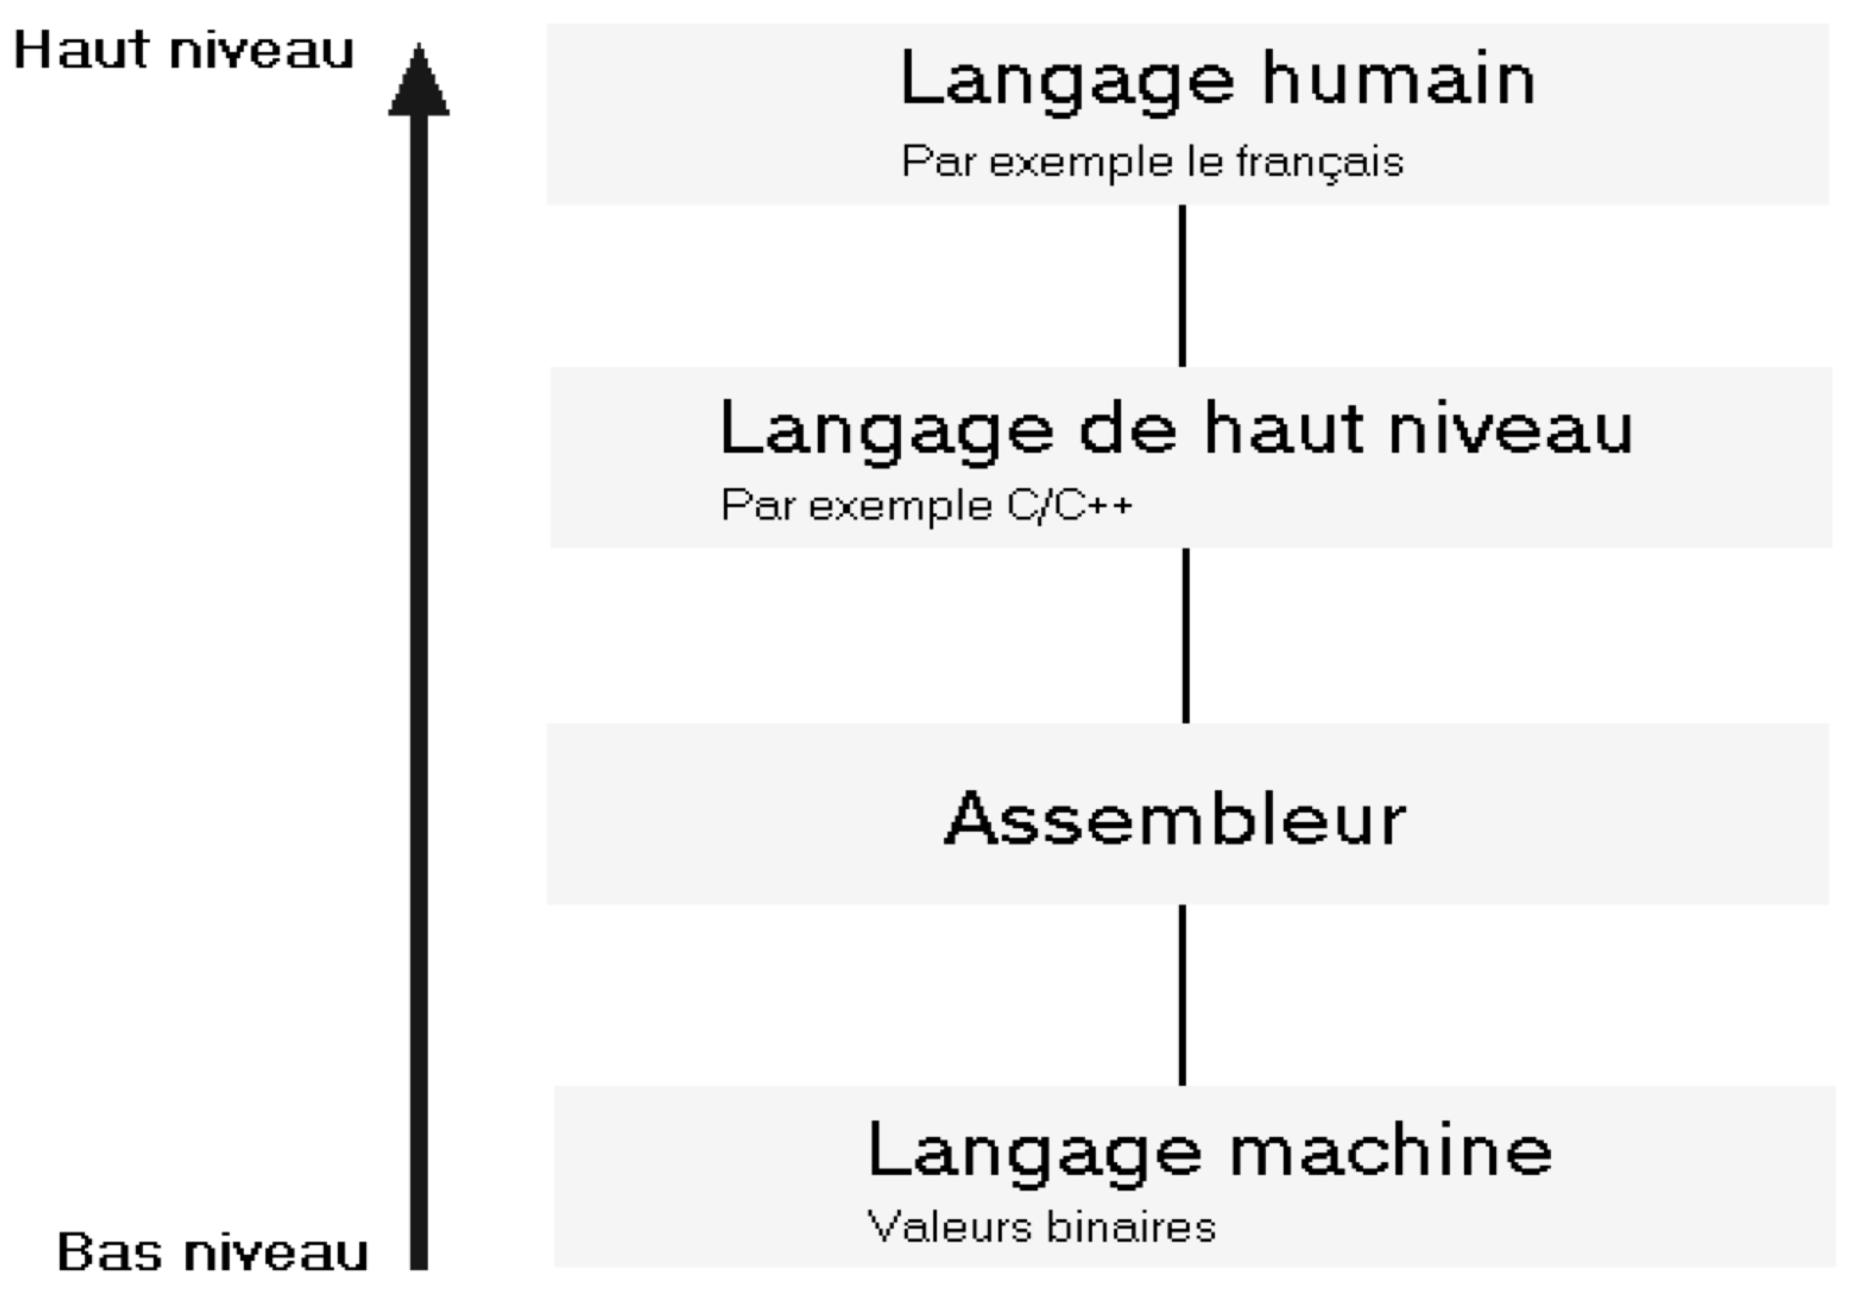
\includegraphics[scale=0.2]{001_LangProg.png}
	\end{figure}
	
	\begin{itemize}
		\item Un langage de programmation...
		
		\begin{itemize}
			\item Comporte une syntaxe, du vocabulaire, une grammaire... comme une langue humaine.
			\item A l'inverse d'une langue humaine ils n'ont qu'une vocation très étroite: écrire des algorithmes de manière à ce qu'un ordinateur puisse les exécuter.
			\item La traduction vers le langage machine que comprend l'ordinateur peut se faire de deux manière:
			
			\begin{itemize}
				\item La compilation  l'équivalent de la traduction d'un livre \textemdash\ cela produit un nouveau fichier, appelé "exécutable" qui peut être directement exécuté par l'ordinateur (comme un livre traduit peut être directement lu).
				\item L'interprétation: comme "dans la vraie vie" c'est une traduction au fur et à mesure que le code est écrit, sans enregistrement du code traduit dans un nouveau fichier.
			\end{itemize}
			\item Exemples:
			
			\begin{itemize}
				\item Le langage C utilise un compilateur \textemdash\ on dit que c'est un langage compilé.
				\item Le langage Python utilise un interpréteur \textemdash\ on dit que c'est un langage interprété.
			\end{itemize}
		\end{itemize}
	\end{itemize}
		
	\pagebreak
		
	\section{Le langage Python \textemdash\ premier contact}
	
	\subsection{A propos de Python...}
	\subsubsection*{Pourquoi est-il celui que l'on étudie ici?}
	\begin{itemize}
		\item A notre niveau pour commencer:
		
		\begin{itemize}
			\item Il est "open source" \textemdash\ gratuit et utilisable par tous.
			\item Il est "portable" \textemdash\ utilisable sous Linux, MacOS, Windows.
			\item Il a une syntaxe simple (\textit{si ! si !}).
		\end{itemize}
		\item Il a d'autres caractéristiques dont nous parlerons quand nous aborderons les thèmes qui y correspondent:
		
		\begin{itemize}
			\item Il gère lui-même ses ressources mémoire.
			\item Il est multi-paradigmes: impératif, fonctionnel, orienté objet.
		\end{itemize}
	\end{itemize}
	\subsubsection*{Comment et où l'utiliser?}
	On le comprend \textemdash\ taper du code dans un fichier texte ne suffit pas à créer un programme (même dans le cas du HTML qu'on a vu la semaine passée, il y avait un interpréteur \textemdash\ le navigateur).

	On va utiliser ce qu'on appelle un IDE ("integrated development environment") \textemdash\ il en existe littéralement des dizaines. On peut citer, pour les plus proches de nous:
		
	\begin{itemize}
		\item IDLE \textemdash\ qui est installé sur les machines NSI et que l'on va utiliser pour découvrir la console;
		\item Basthon \textemdash\ outil en ligne sur lequel s'appuie l'application Capytale que nous allons utiliser bientôt également;
		\item EduPython \textemdash\ qui est installé sur les machines qui vous ont été fournies par la Région Ile-de-France;
		\item Google Colab \textemdash\ outil en ligne que l'on utilisera sans doute plus tard dans l'année.
	\end{itemize}
	
	\subsection{Python comme calculatrice}
	{\large \faLightbulbO} \hspace{1cm} Dans ce document tous les encadrés à bordure rouge tels que celui ci-dessous dénotent une activité que nous avons réalisée en classe \textemdash\ et que vous devriez donc pouvoir retrouver dans votre ENT.
	
	\begin{tcolorbox}[colframe=red!75!black, boxrule=2pt]
		\begin{minipage}{1\textwidth}
			\begin{itemize}				
				\item Lancer IDLE
				\item Testez dans la console les opérations arithmétiques usuelles: \texttt{+  -  *  /}
			\end{itemize}
			{\footnotesize 			\texttt{>>> 3 + 2}
			
			\texttt{5}
			
			\texttt{>>> 9 / 5}
			
			\texttt{1.8}
			
			\texttt{>>>}}

			\begin{itemize}
				\item Testez les opérations \texttt{//} et \texttt{\%} \textemdash\ devinez-vous ce qu'elles font?
			\end{itemize}
		\end{minipage}
	\end{tcolorbox}
	
	\subsection{Entrées \& sorties; affectations}
	\noindent
	\framebox{\parbox{\dimexpr\linewidth-2\fboxsep-2\fboxrule}{Une \textbf{variable} est une manière de stocker une information dans la machine en la nommant.}}
	\\
	\\
	\\
	\framebox{\parbox{\dimexpr\linewidth-2\fboxsep-2\fboxrule}{Faire \textbf{l'affectation} d'une variable c'est en modifier la valeur \textemdash\  soit en la \textit{créant} si elle n'existe pas encore, soit en la \textit{changeant}.}}
	\\
	\\
	\\
	Considérons l'algorithme suivant:
	\nopagebreak
	\begin{listing}[H]
		\inputminted
		[
			bgcolor = gray!15, % pas essentiel
			fontsize = \footnotesize,
			linenos = true % numéros de ligne
		]
		{python}
		{_code/001_AlgoInit.py}
	\end{listing}

	\noindent
	On a ici:
	
	\begin{itemize}
		\item Trois variables;
		\item Deux entrées;
		\item Quatre affectations (deux sur des valeurs demandées à l'utilisateur, deux calculées par l'ordinateur);
		\item Une sortie, par écriture à l'écran.
	\end{itemize}

	
	\noindent
	\begin{wrapfigure}{r}{0.5\textwidth}
		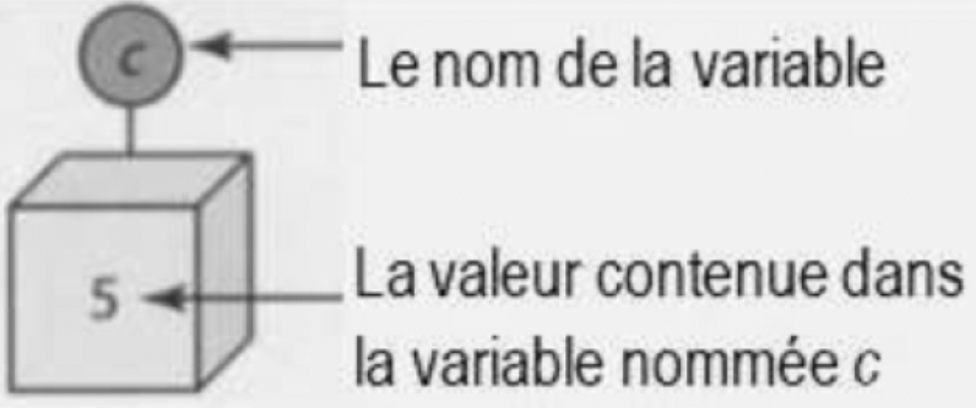
\includegraphics[scale=0.4]{002_Affectation.png}
	\end{wrapfigure}
	Une variable est caractérisée en premier lieu par un nom (qui permet de la localiser en mémoire) et une valeur; elle peut être vue comme une boîte étiquetée (son nom) qui peut contenir différentes informations (sa valeur) --- dans le cas précédent, des nombres entiers. Affecter une variable, c'est modifier ce que contient la boîte.	

	Une variable a également un type --- nombre entier, nombre réel, chaîne de caractères... --- mais à l'inverse d'autres langages, il est implicite : il n'y a pas besoin de le déclarer.
	
	Pour affecter une valeur à une variable en Python, on utilise le symbole \texttt{=}, le membre de gauche prenant la valeur de celui de droite :
	
	\begin{minted}
		[
		bgcolor = gray!15, % pas essentiel
		fontsize = \footnotesize,
		linenos = false % numéros de ligne
		]
		{python}
# La ligne suivante affecte la valeur 3 a "variable"
variable = 3
	\end{minted}
	{\large \faLightbulbO} \hspace{1cm} \textit{On notera ici la syntaxe des commentaires en Python (que j'espère que vous utiliserez beaucoup!!) qui sont préfixés par un "hashtag".}
	
	\textbf{ATTENTION} à ne pas confondre avec les maths:
	
	\begin{itemize}
		\item "Variable" n'a pas le même sens;
		\item Le symbole "\texttt{=}" n'a pas le même sens.
	\end{itemize}

	Pour nommer une variable, il faut respecter certaines règles: 
	\begin{itemize}
		\item Caractères alphanumériques;
		\item Ne pas commencer par un chiffre;
		\item Aucun caractère spécial hormis l'underscore "\_";
		\item On évite les accents - même si en principe ils ne sont pas interdits;
		\item Et les mots clés --- int, and, break... --- sont interdits (on y reviendra).
	\end{itemize}

	\begin{tcolorbox}[colframe=red!75!black, boxrule=2pt]
	\begin{minipage}{1\textwidth}
		\begin{itemize}				
			\item Créez plusieurs variables et affectez-y différentes valeurs, cette fois de différents types (entiers, réels, texte...). (vous pouvez utiliser les exemples ci-dessous --- mais inventez-en d'autres!)
		\end{itemize}
			\begin{minted}
			[
			bgcolor = gray!15, % pas essentiel
			fontsize = \footnotesize,
			linenos = false % numéros de ligne
			]
			{python}
# Quelques exemples d'affectations pour s'entrainer...
MaVariable = 5
Fustel = 6.578
accueil = "bonjour"
			\end{minted}
			\begin{itemize}
				\item Affichez la valeur de ces variables au moyen de la fonction:
			\end{itemize}
			\centering
			\texttt{print()}
			\begin{itemize}
				\item Demandez à l'utilisateur de renseigner certaines variables au moyen de la fonction input:
			\end{itemize}
			\centering
			\texttt{age\_prof = "Quel âge avez-vous?   "}
			\begin{itemize}
				\item Vérifiez le type des variables que vous avez créé au moyen de la commande :
			\end{itemize}
			\centering
			\texttt{print(type(NOM\_VARIABLE))}
			\begin{itemize}
				\item On rappelle les opérations usuelles:
			\end{itemize}
			\begin{tabular}{|c|c|}
				\hline
				\textbf{Instruction} & \textbf{Signification} \\
				\hline
				\texttt{a + b} & addition \\
				\texttt{a - b} & soustraction \\
				\texttt{a * b} & multiplication \\
				\texttt{a ** b} & puissance:  $a^b$\\
				\texttt{a / b} & division \\
				\texttt{a // b} & division entière (quotient de la divition euclidienne) \\
				\texttt{a \% b} & modulo (reste de la divition euclidienne) \\
				\hline
			\end{tabular}
			\begin{itemize}
				\item Faites des tests d'opérations usuelles avec l'ensemble des variables que vous avez affectées précédemment --- rencontrez-vous des erreurs? Lesquelles?
			\end{itemize}
		\end{minipage}
	\end{tcolorbox}
	
	\subsubsection*{Exercices}
	On considère le programme Python suivant:
	\begin{minted}
		[
		bgcolor = gray!15, % pas essentiel
		fontsize = \footnotesize,
		linenos = true % numéros de ligne
		]
		{python}
a = 7
b = 3
c = a + b
c = c + 1
b = a - c
	\end{minted}
	Sur une feuille copiez le tableau suivant et complétez-le:
	
	\begin{tabular}{|c|c|c|c|}
		\hline
		\textbf{Contenu variables en...} & \textbf{a} & \textbf{b} & \textbf{c} \\
		\hline
		Ligne 1 & \hspace*{0.7cm} & \hspace*{0.7cm} & \hspace*{0.7cm} \\
		\hline
		Ligne 2 & & & \\
		\hline
		Ligne 3 & & & \\
		\hline
		Ligne 4 & & & \\
		\hline
		Ligne 5 & & & \\
		\hline
	\end{tabular}
	
	\textit{Correction du QCM que vous avez fait sur ProNote:}
	\nopagebreak
	\begin{figure}[H]
		\centering
		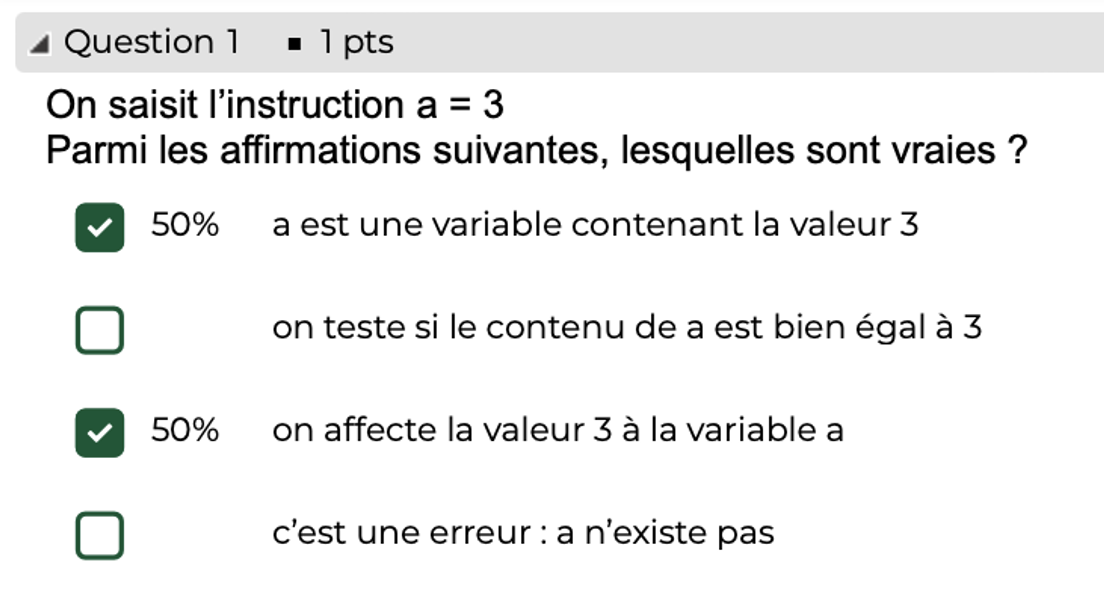
\includegraphics[scale = 0.5]{003_QCM_Q1.png}
	\end{figure}
	\begin{figure}[H]
		\centering
		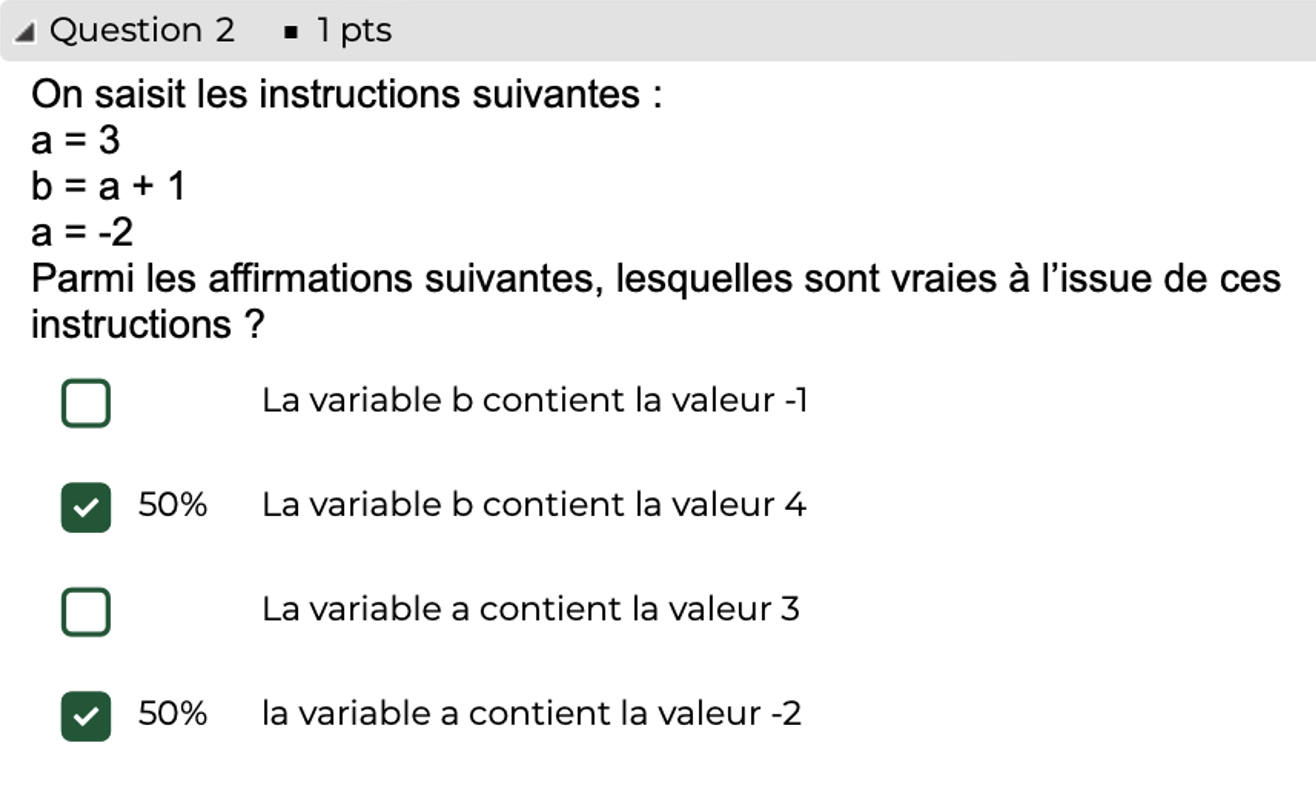
\includegraphics[scale = 0.5]{004_QCM_Q2.png}
	\end{figure}
	\begin{figure}[H]
		\centering
		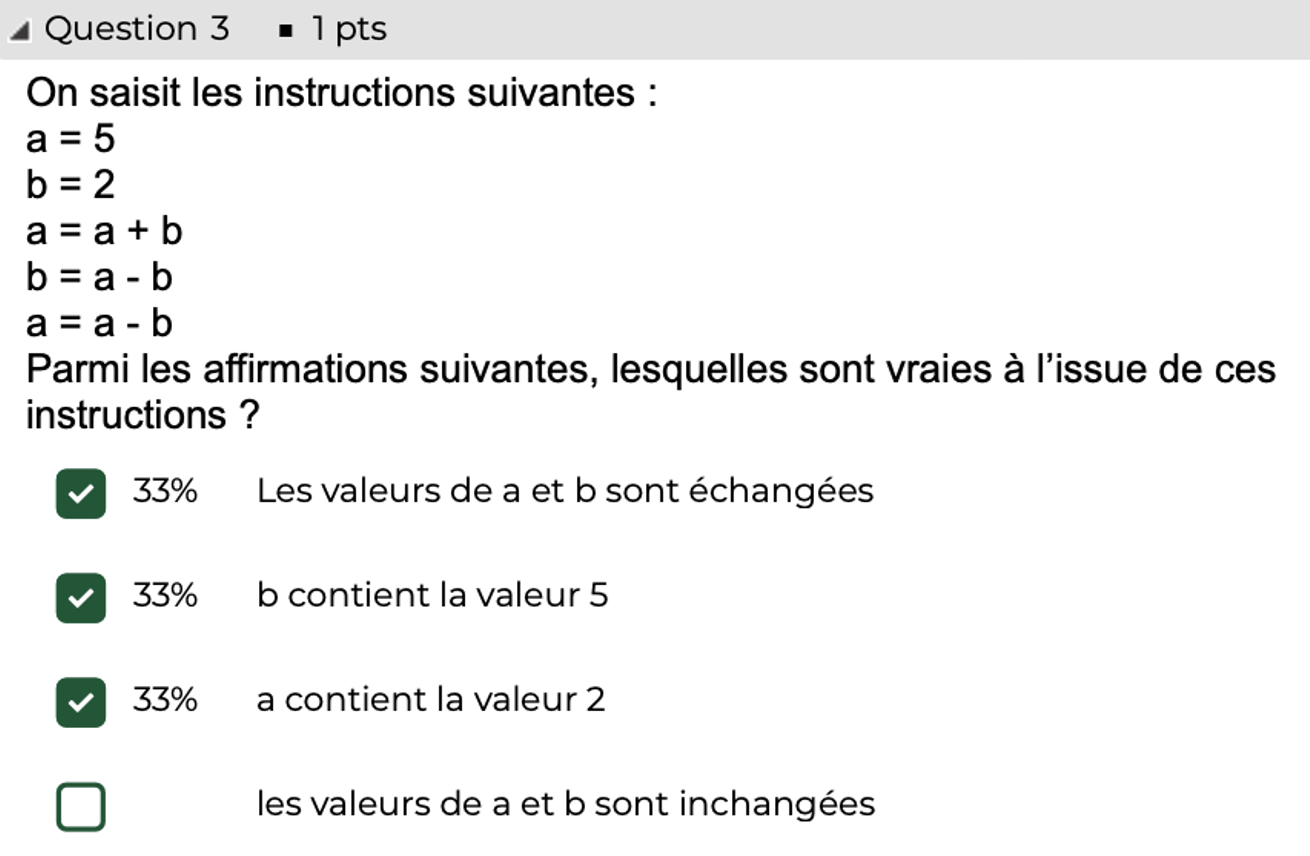
\includegraphics[scale = 0.5]{005_QCM_Q3.png}
	\end{figure}

	\subsection{Les scripts}
	
	Un script n'est rien de plus qu'\textbf{une succession d'instructions} qui sont exécutées à la suite --- dans une console chaque instruction est exécutée lorsque vous passez à la ligne suivante tandis que dans un script elles le sont toutes sans que vous n'ayez rien à faire pour passer de l'une à la suivante.
	
	Un script peut être \textbf{enregistré} pour être \textbf{exécuté plusieurs fois} ou dans plusieurs contextes ---c'est, au sens où il contient une suite d'instructions mettant en œuvre un algorithme, réellement un \textbf{"programme informatique"}.
	
		\begin{tcolorbox}[colframe=red!75!black, boxrule=2pt]
		\begin{minipage}{1\textwidth}
			\begin{itemize}				
				\item Depuis votre ENT, lancez l'application "Capytale".
				\item Avant de vous lancer n'oubliez pas qu'avec Python on peut convertir (quand c'est possible) des variables d'un type à un autre:
			\end{itemize}
			\begin{minted}
				[
				bgcolor = gray!15, % pas essentiel
				fontsize = \footnotesize,
				linenos = false % numéros de ligne
				]
				{python}
# Mettre un nombre au format chaine de caracteres (string)
a = 1984
b = str(a)
c = "Roman de Orwell: " + b
# Ou au contraire:
a = input("Quel est votre age?   ")
b = int(a)
print(b + 10)
# Ou encore en float...
a = input("Que vaut pi avec deux decimales?")
b = float(a)
aire2 = b * 2 ** 2
			\end{minted}
			\begin{itemize}
				\item Rejoignez l'activité que j'ai préparée pour la séance avec le code:
			\end{itemize}
			\centering
			\textbf{\texttt{d00f-1846631}}
		\end{minipage}
	\end{tcolorbox}
	
	\subsection{Introduction aux notebooks Jupyter}
	\begin{itemize}
		\item Les notebooks Jupyter sont des cahiers électroniques qui, dans le même document, peuvent rassembler du texte, des images, des formules mathématiques et du code informatique exécutable. Ils sont manipulables interactivement dans un navigateur web.
		\item Ces notebooks sont organisés en cellules qui peuvent être soit du texte (auquel cas on peut y inclure des images ou des formules également) soit du code Python (pour ce cours en tous cas).
		\item Ces notebooks sont facilement convertibles au format PDF en ligne --- ce qui permet de réellement s'en servir comme d'un bloc-notes.
		\item Tout se passe comme si les cellules de code étaient dans des terminaux les uns à la suite des autres --- mais entre elles je peux mettre des instructions et vous pouvez prendre des notes!
	\end{itemize}

	\begin{figure}[H]
		\centering
		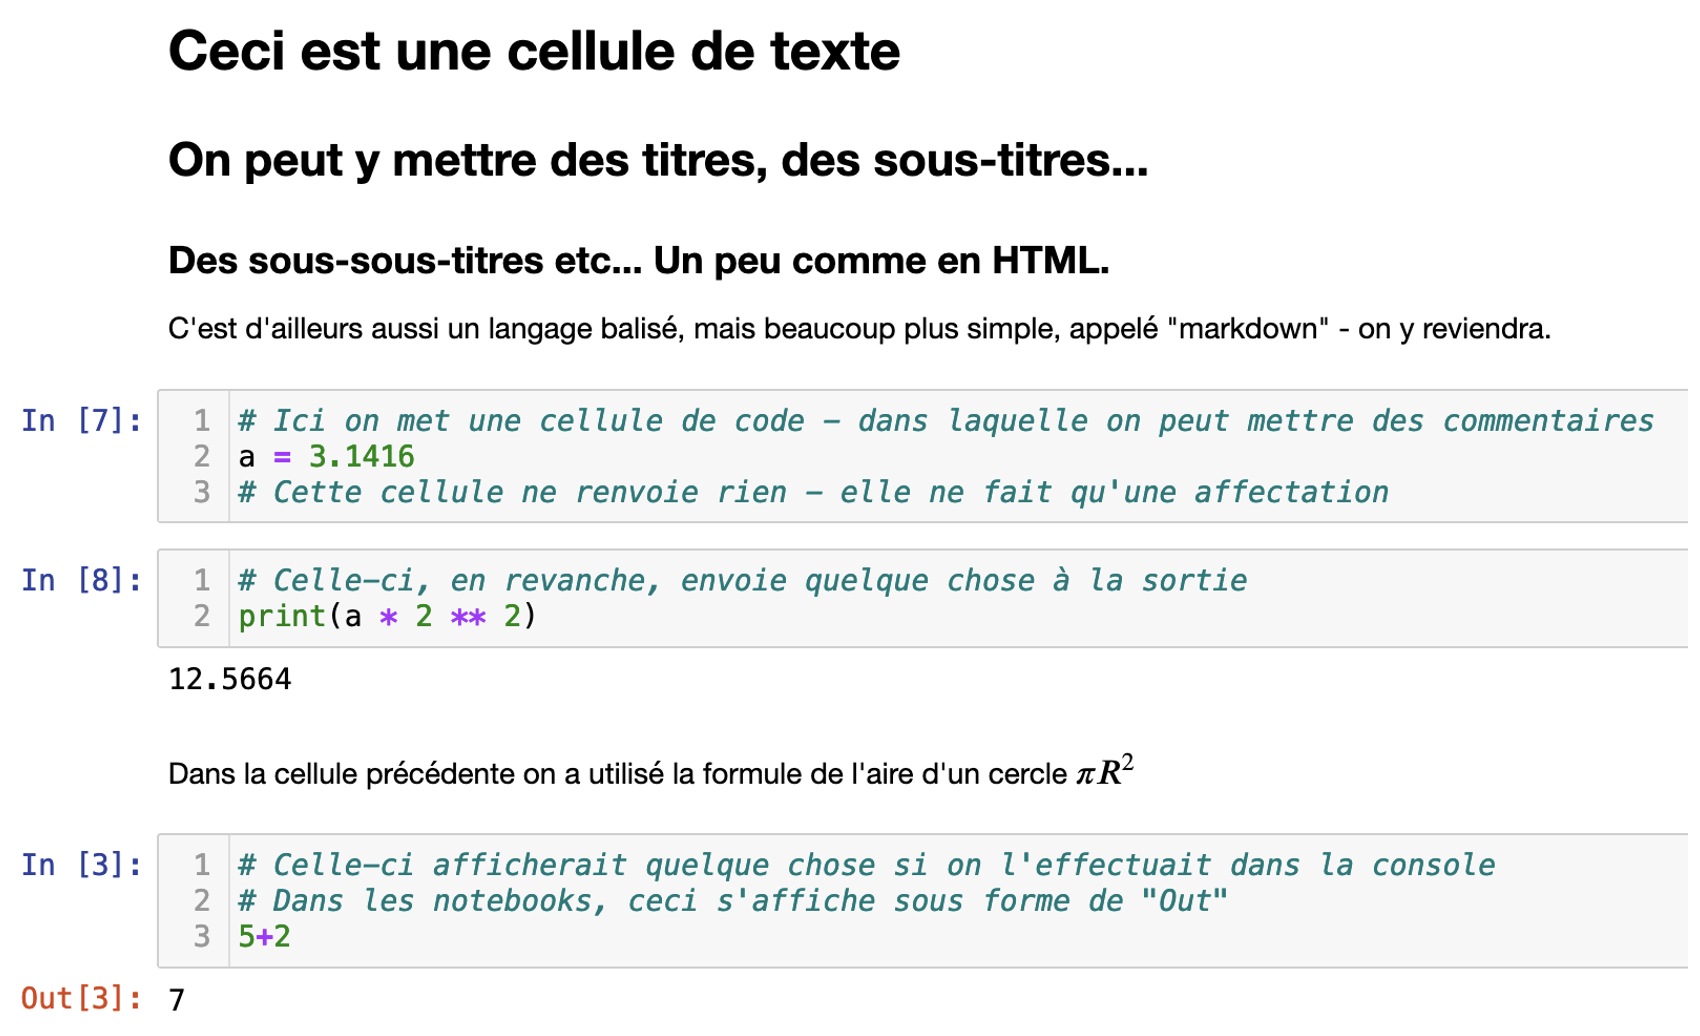
\includegraphics[width=\textwidth]{006_Jupyter.png}
	\end{figure}
	
	\begin{tcolorbox}[colframe=red!75!black, boxrule=2pt]
		\begin{minipage}{1\textwidth}
			\begin{itemize}				
				\item Depuis votre ENT, lancez l'application "Capytale".
				\item Rejoignez l'activité que j'ai préparée pour la séance avec le code:
			\end{itemize}
			\centering
			\textbf{\texttt{ab1d-1883830}}
		\end{minipage}
	\end{tcolorbox}
	\leavevmode
	\\
	
	\noindent
	\framebox{\parbox{\dimexpr\linewidth-2\fboxsep-2\fboxrule}{\centering \textbf{A partir de maintenant nous allons régulièrement utiliser ce format pour les TPs --- alors prenez-soin de bien vous y habituer!}}}
	
	\pagebreak
	
	\section{Programmation en Python}
	
	\subsection{Fonctions}
	\textit{Attention pour commencer}: comme pour le "\texttt{=}" et pour la notion de variable, le mot "fonction" n'a pas le même sens en mathématiques et en informatique: dans le premier cas c'est \textit{une relation entre deux ensembles}, dans le second \textit{un procédé de calcul} --- comme nous allons le découvrir.
	
	\noindent
	\framebox{\parbox{\dimexpr\linewidth-2\fboxsep-2\fboxrule}{
			Une \textbf{fonction}:
			\begin{itemize}
				\item Est définie par un \textbf{nom};
				\item Correspond à une \textbf{séquence d'instructions} réalisant une tâche précise;
				\item Utilise aucun, un, ou plusieurs "\textbf{arguments}". Ces arguments sont les paramètres que la fonction reçoit en entrée;
				\item Renvoie généralement \textbf{un résultat}; si elle ne le fait pas, on parle d'une \textbf{procédure}.
			\end{itemize}
		}}
	
	Les fonctions ont plusieurs utilités:
	\begin{itemize}
		\item Décomposition d'une tâche complexe:
	\end{itemize}
	\begin{figure}[H]
		\centering
		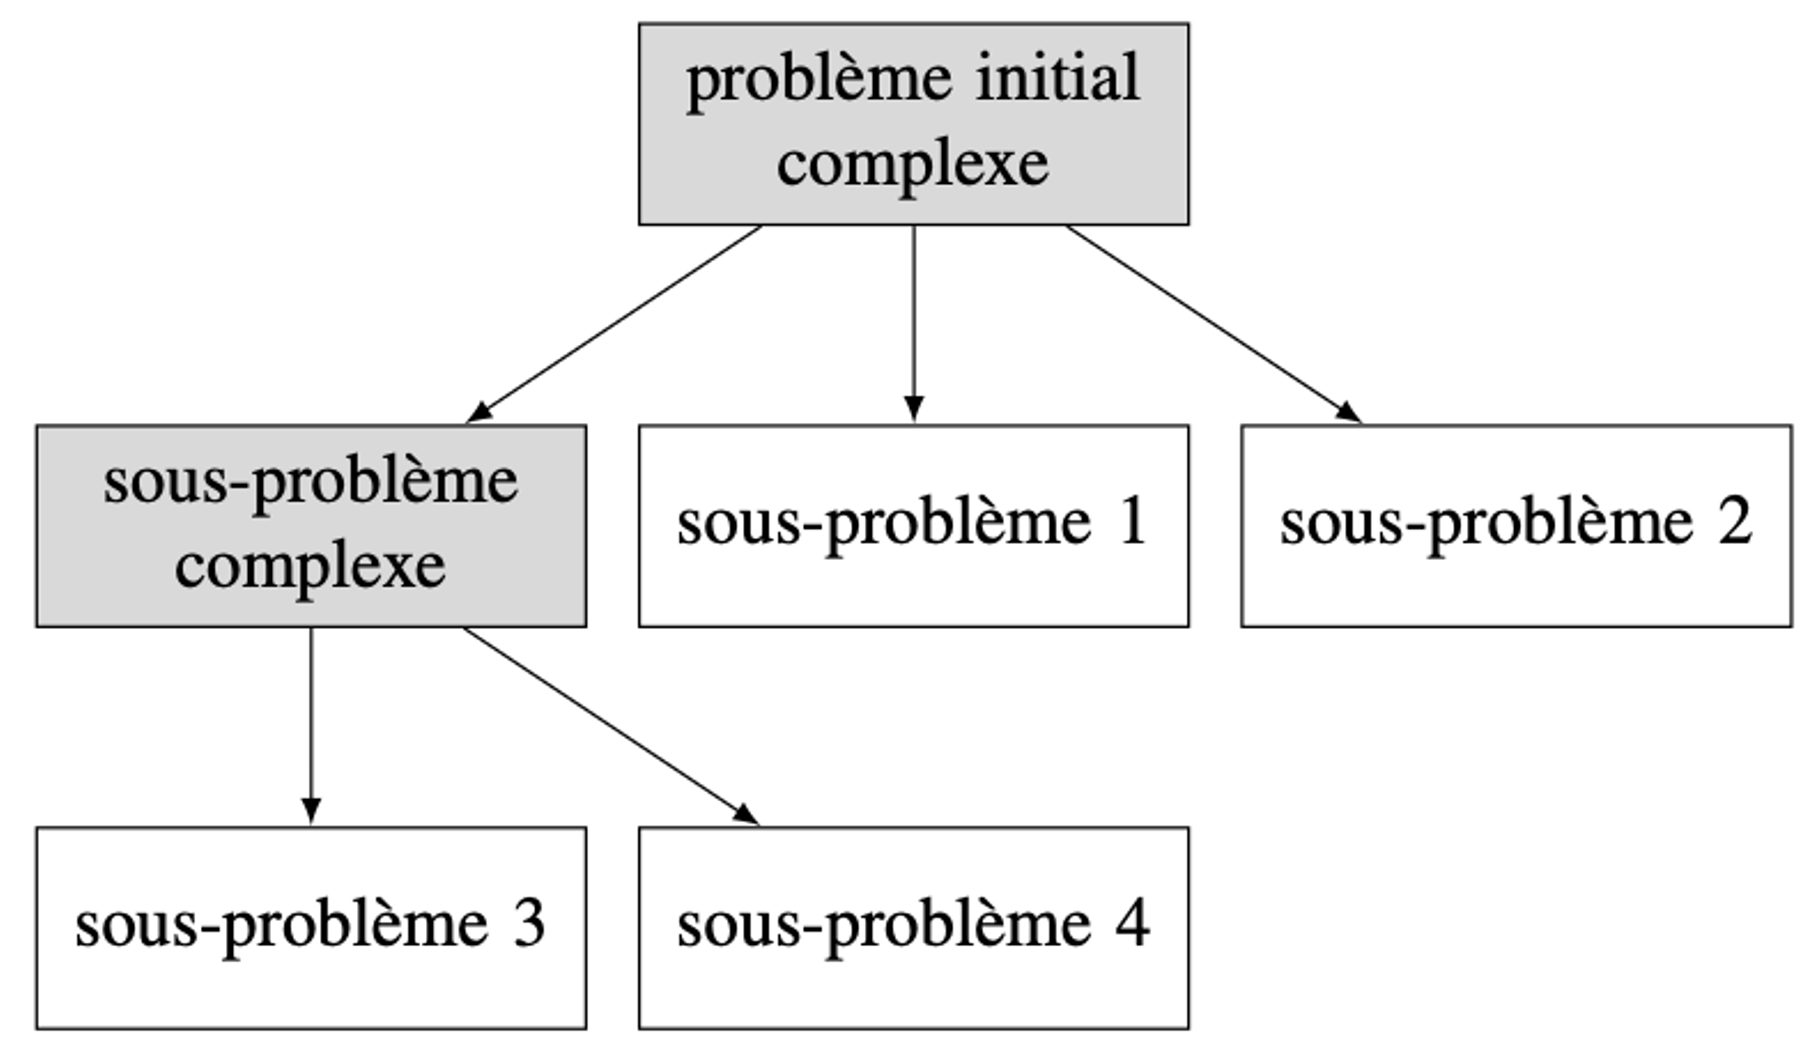
\includegraphics[scale=0.3]{007_FoncDecomp.png}
	\end{figure}
	\begin{itemize}
		\item Réutilisation de code / éviter les répétitions:
	\end{itemize}
	\begin{figure}[H]
	\centering
	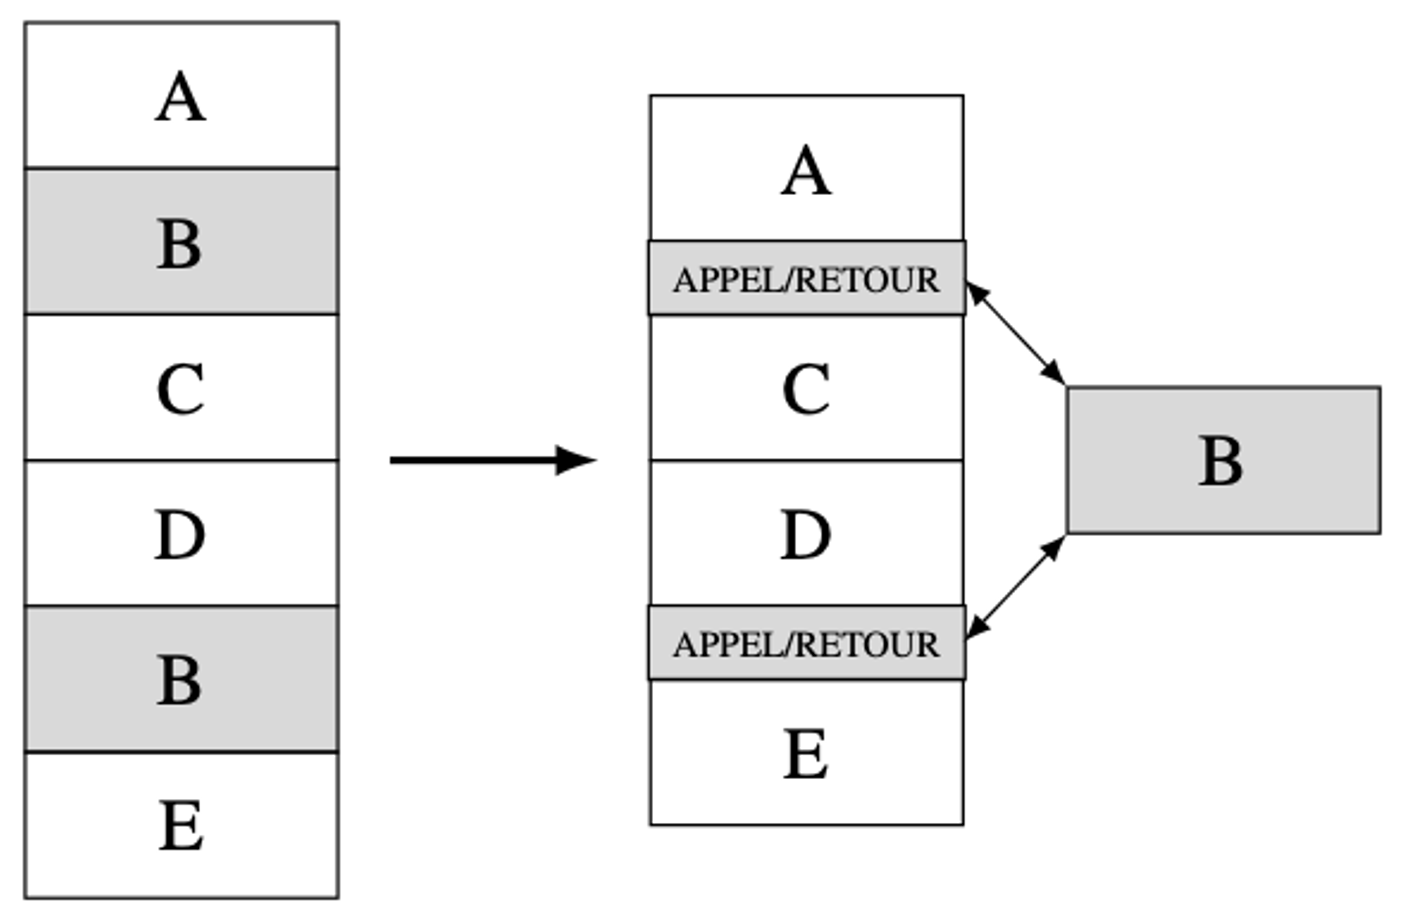
\includegraphics[scale=0.3]{008_FoncReutil.png}
	\end{figure}
	\begin{itemize}
		\item En conséquence: rendre le code plus court et lisible.
	\end{itemize}
	
	\subsubsection*{Syntaxe en Python:}
	\nopagebreak
	\begin{minipage}{0.67\textwidth}
		\begin{lstlisting}
# Definition de la fonction
def nom_fonction(liste_parametres):
	<bloc d'instuctions>
	return resultat

# Appel d'une fonction
resultat = nom_fonction(parametres)

# Appel d'une procedure
nom_procedure(parametres)

		\end{lstlisting}
	\end{minipage}
	\begin{minipage}{0.3\textwidth}
		
\includegraphics[scale=0.25]{009_Indentation.png}
	\end{minipage}
	
	Considérons le code suivant:
	\begin{listing}[H]
		\inputminted
		[
		bgcolor = gray!15, % pas essentiel
		fontsize = \footnotesize,
		linenos = true % numéros de ligne
		]
		{python}
		{_code/002_ConvMinutes.py}
	\end{listing}
	
	Vérifiez que ce code affichera à l'utilisateur:
	
	\begin{center}
		\textbf{\texttt{2 heures 30 font 150 minutes}}
	\end{center}
	
	Note: lorsqu'une fonction est appelée, Python réserve pour elle (dans la mémoire de l'ordinateur) \textbf{un espace de noms}. Cet espace de noms local à la fonction est différent de l'espace de noms global où se trouvent les variables du programme principal. Dans l'espace de noms local, nous aurons des variables qui ne sont accessibles qu'au sein de la fonction --- on parle alors de \textbf{variables locales}.
	
	\begin{tcolorbox}[colframe=red!75!black, boxrule=2pt]
		\begin{minipage}{1\textwidth}
			\begin{itemize}				
				\item Rendez-vous sur \href{https://pythontutor.com}{https://pythontutor.com}.
				\item Cliquer sur "Python".
				\item Écrire le code suivant:
			\end{itemize}
			\begin{minted}
				[
				bgcolor = gray!15, % pas essentiel
				fontsize = \footnotesize,
				linenos = false % numéros de ligne
				]
				{python}
def conv_minutes(heures, minutes):
    minutes = minutes + heures * 60
    return minutes

heures = 2
minutes = 30
resultat = conv_minutes(heures, minutes)

print("2 heures 30 font ", resultat, " minutes.")
			\end{minted}
			\begin{itemize}
				\item Cliquer sur Visualize Execution et exécuter la fonction pas à pas.
				\item Ouvrez IDLE.
				\item Écrivez une fonction perimetre\_rectangle qui prend en argument deux paramètres --- une longueur et une largeur --- et qui renvoie le périmètre du rectangle.
				\item Exécutez-là plusieurs fois et observez les sorties:
			\end{itemize}
			\textbf{\texttt{perimetre\_rectangle}}\\
			\textbf{\texttt{perimetre\_rectangle()}}\\
			\textbf{\texttt{perimetre\_rectangle(3, 5)}}\\
			\textbf{\texttt{perimetre\_rectangle(10, 2)}}\\
			\textbf{\texttt{perimetre\_rectangle(9)}}
		\end{minipage}
	\end{tcolorbox}
	
	Pour rappel, ce que vous affiche PythonTutor dans ce cas ressemble à ceci:
	
	\begin{figure}[H]
		\centering
		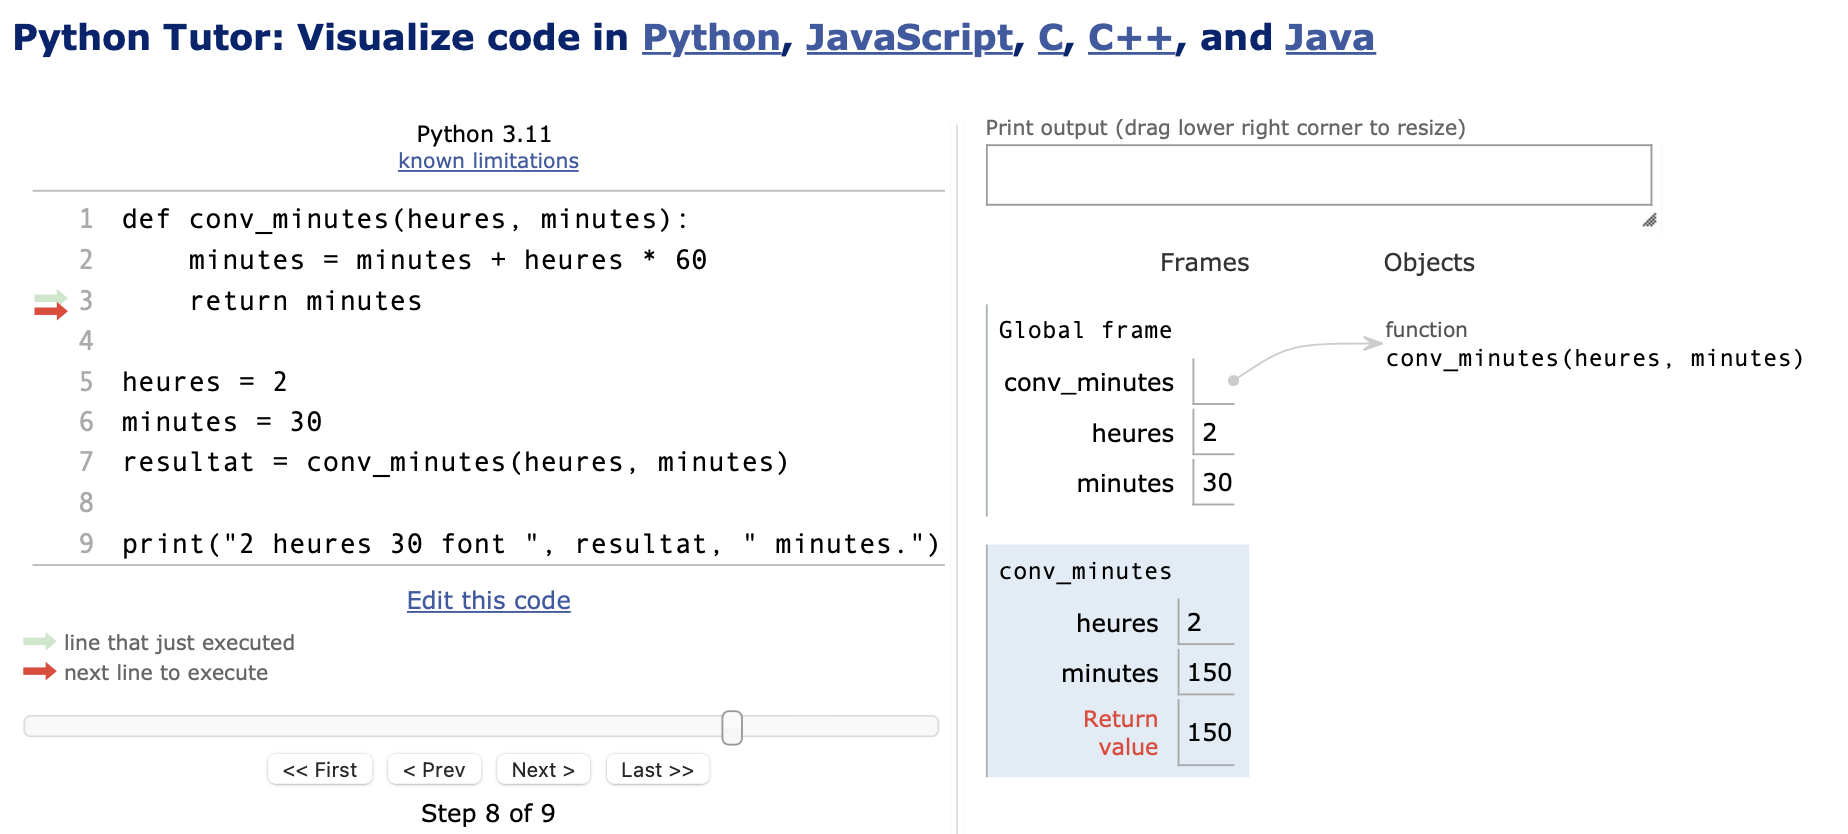
\includegraphics[width=\textwidth]{010_PythonTutor.png}
	\end{figure}
	
	\noindent
	\framebox{\parbox{\dimexpr\linewidth-2\fboxsep-2\fboxrule}{\centering \textbf{N'hésitez pas à utiliser Python Tutor régulièrement pour visualiser l'organisation de l'utilisation de la mémoire par Python dans les programmes que vous développez --- vous verrez, ça vous éclairera souvent sur des bugs que vous ne comprenez pas!}}}
	
	\subsection{Conditions \& Embranchements}
	\nopagebreak
	\subsubsection*{Introduction}
	\nopagebreak
	Situations classiques de la vie courante --- \textit{je dois sortir...}
	\nopagebreak
	\begin{figure}[H]
		\centering
		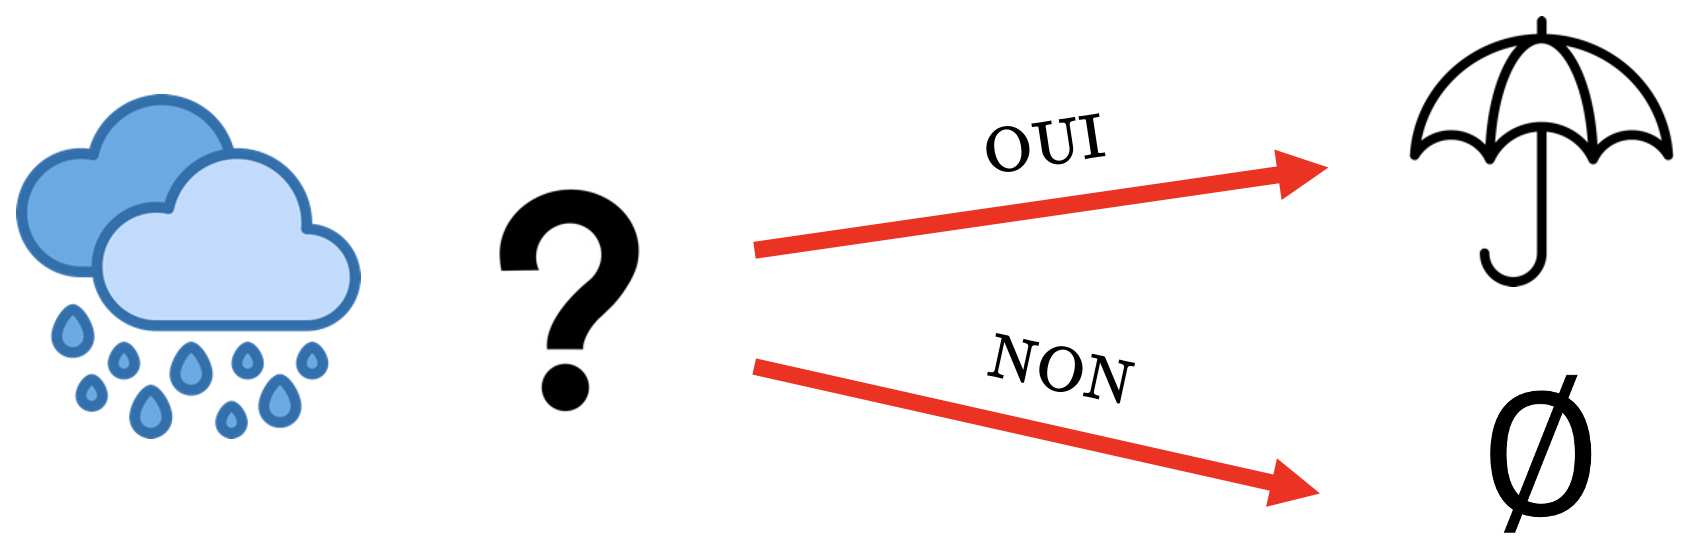
\includegraphics[width=\textwidth]{011_ConditionPluie.png}
	\end{figure}
	
	On a mis en place une \textbf{condition} ("s'il pleut") et une \textbf{structure d'embranchement} (ce que je fais dans un cas; ce que je fais sinon).
	
	\noindent
	\begin{wrapfigure}{l}{0.3\textwidth}
		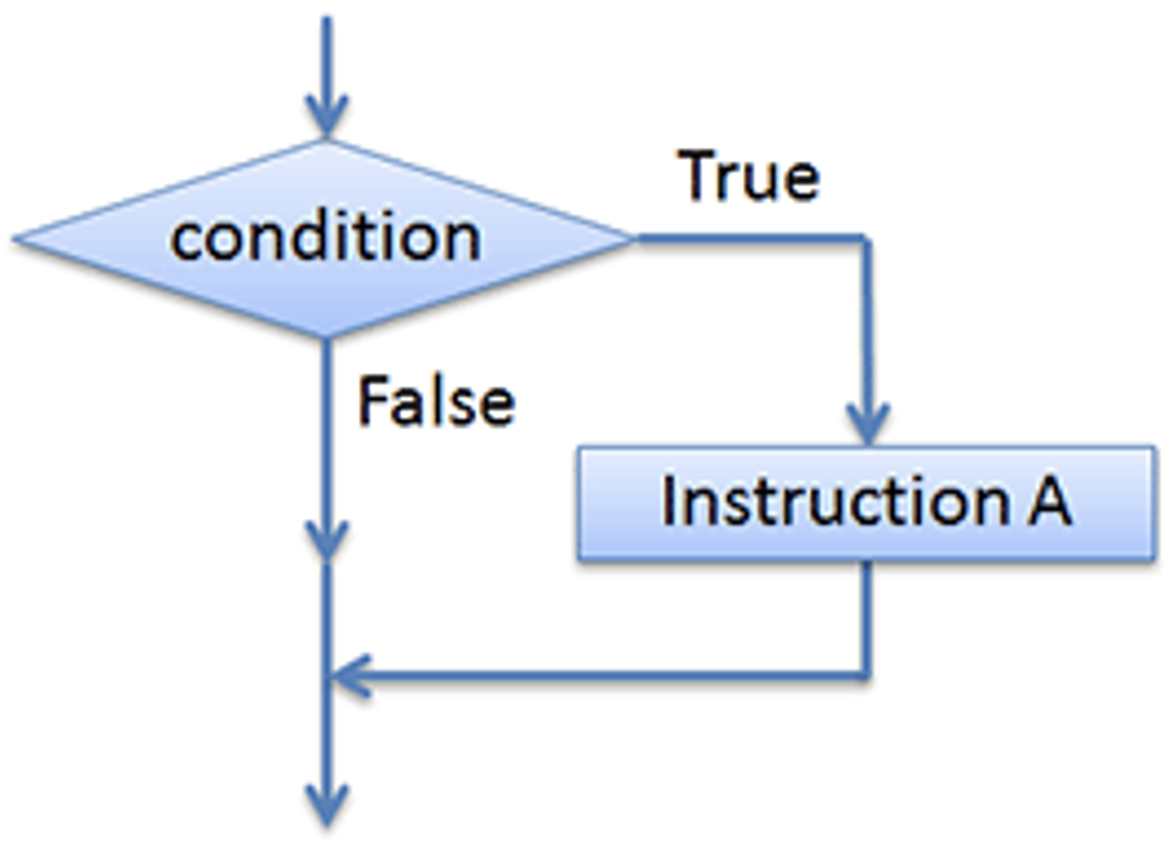
\includegraphics[scale=0.20]{012_IfThen.png}
	\end{wrapfigure}
	
	Remarque: une structure d'embranchement, dans la vie courante comme en programmation, une fois résolue, revient à la poursuite "normale" des actions. Ici :
	\begin{itemize}
		\item S'il pleut --- \textit{alors} je prends mon parapluie, \textit{puis} je sors.
		\item S'il ne pleut pas --- \textit{alors} je ne fais rien de spécial, \textit{puis} je sors.
	\end{itemize}
		
	\subsubsection*{Conditions et tests:}
	\framebox{\parbox{\dimexpr\linewidth-2\fboxsep-2\fboxrule}{Une \textbf{condition} est:
	\begin{itemize}
		\item Un \textbf{énoncé} qui peut prendre \textbf{deux valeurs et seulement deux valeurs}: Vrai ou Faux.
		\item Sa \textbf{résolution} est donc une \textbf{variable booléenne (True / False)}.
		\item  Une \textbf{combinaison de tests reliés par des opérateurs logiques}.
	\end{itemize}
	}}

	Ces tests sont la plupart du temps réalisés à l’aide d’opérateurs de comparaison dont les plus fréquents sont:	
	
	\begin{tabular}{|c|c|}
		\hline
		\textbf{Opérateur} & \textbf{Signification} \\
		\hline
		\texttt{=} & égal \\
		\texttt{!=} & différent de \\
		\texttt{<=} & inférieur ou égal \\
		\texttt{>=} & supérieur ou égal\\
		\texttt{<} & strictement inférieur \\
		\texttt{>} & strictement supérieur \\
		\hline
	\end{tabular}
	
	Les opérateurs logiques classiques quant à eux sont:
\nopagebreak

	\begin{tabular}{|c|p{0.79\textwidth}|}
		\hline
		\textbf{Opérateur} & \textbf{Signification} \\
		\hline
		\texttt{not} & "non" logique --- négation d’une condition \\
		\hline
		\texttt{or} & "ou" logique --- vrai si une de deux conditions au moins est vraie, faux sinon\\
		\hline
		\texttt{and} & "et" logique --- vrai si les deux conditions sont vraies, faux sinon\\
		\hline
	\end{tabular}
	
	\begin{tcolorbox}[colframe=red!75!black, boxrule=2pt]
		\begin{minipage}{1\textwidth}
			\begin{itemize}				
				\item Lancer IDLE
				\item Testez dans la console différentes conditions combinant les éléments précédents --- par exemple:
			\end{itemize}
			{\footnotesize 
				\texttt{>>> a = 4}
				
				\texttt{>>> b = 5}
				
				\texttt{>>> a == 4}
				
				\texttt{>>> a == 4 or b < 10}
				
				\texttt{>>> a == 4 and b < 10}
				
				\texttt{>>> a >= 4 or b == 6}
				
				\texttt{>>> a < 3 and b == 5}
				
				\texttt{>>> not(b == 5)}
			}
		\end{minipage}
	\end{tcolorbox}
	
	\subsubsection*{Embranchements:}
	La syntaxe en python pour réaliser un \textbf{embranchement} simple (tel que l’exemple de la pluie plus haut) est la suivante: 
	
	\begin{figure}[H]
		\centering
		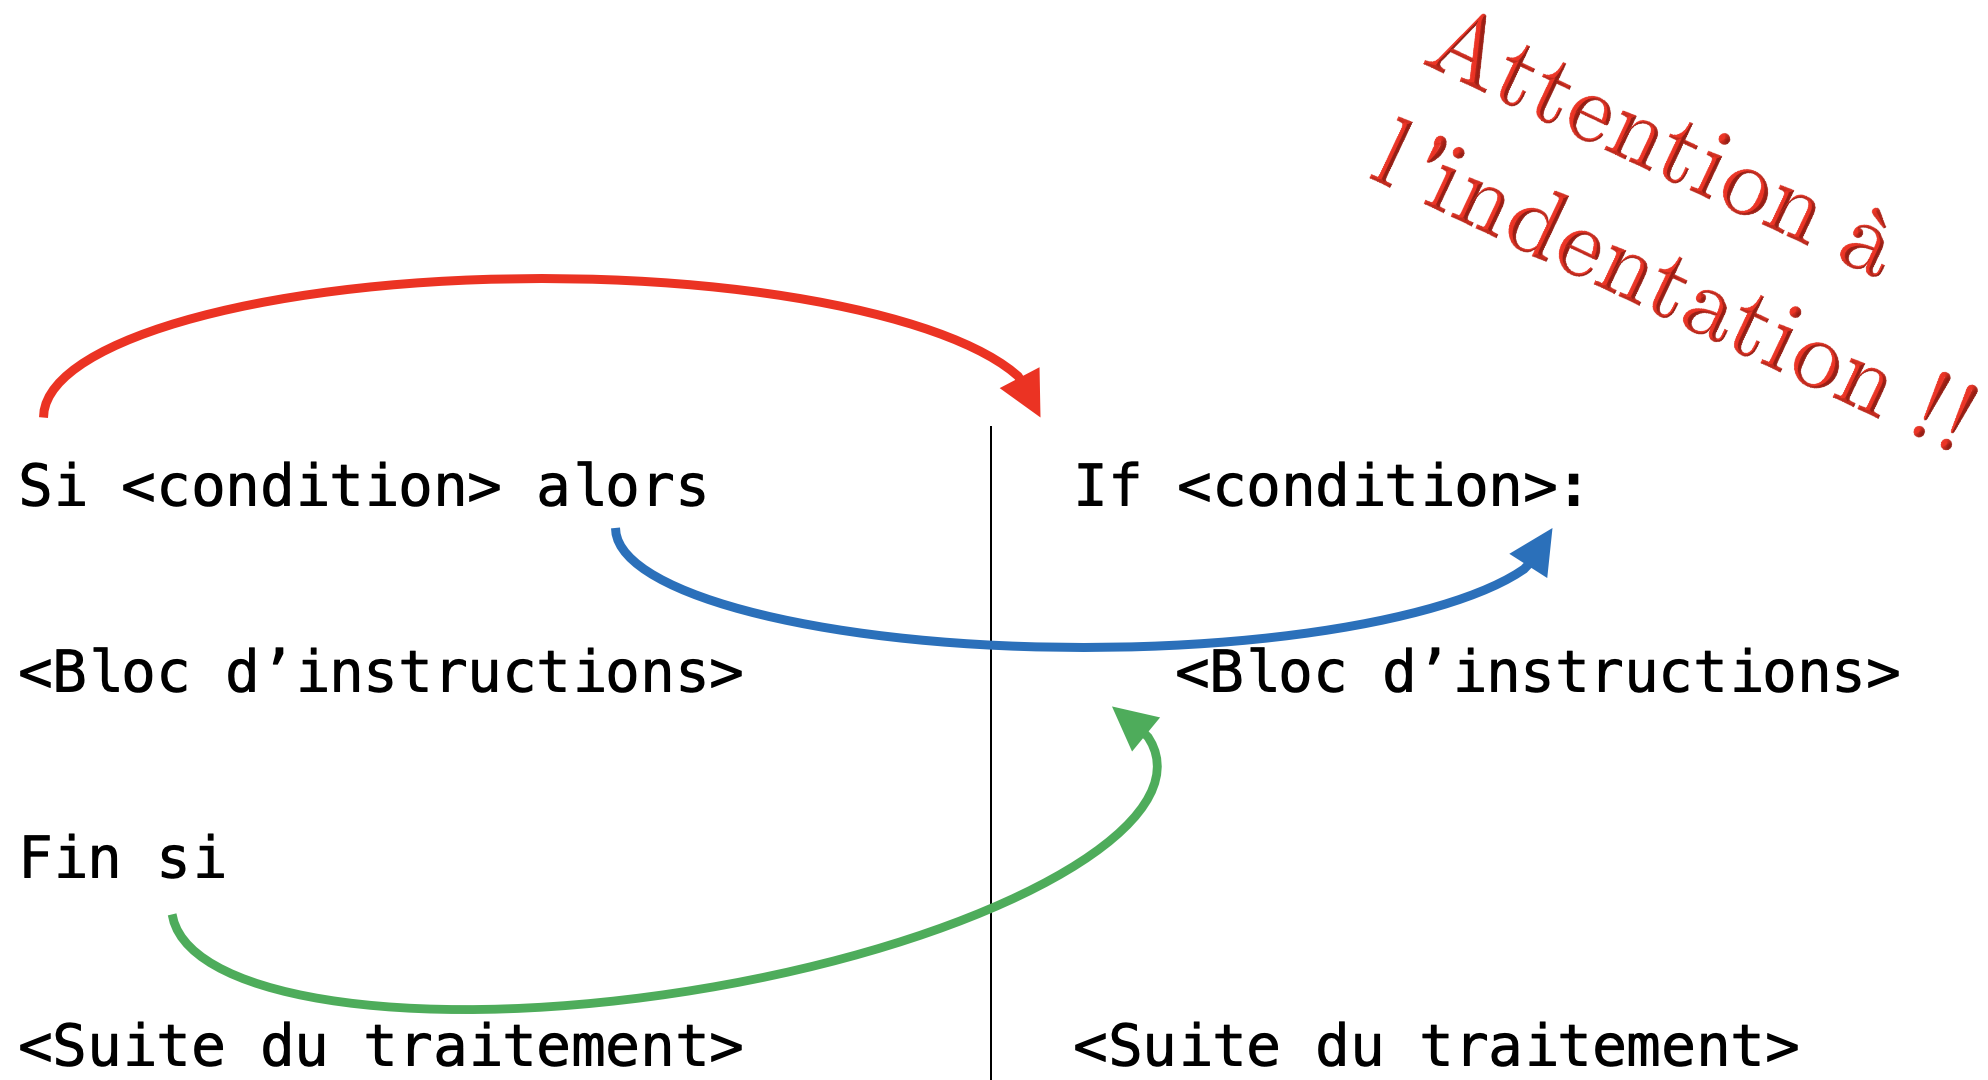
\includegraphics[width=0.7\textwidth]{013_Embranchement.png}
	\end{figure}
	
	\begin{listing}[H]
		\inputminted
		[
		bgcolor = gray!15, % pas essentiel
		fontsize = \footnotesize,
		linenos = true % numéros de ligne
		]
		{python}
		{_code/003_IfThen.py}
	\end{listing}
	Puisque les embranchements ne sont parcourus \textit{que} si la condition est remplie, mais que le corps principal du programme (qui dans ce cas en est la partie non-indentée) l'est dans tous les cas, l'affichage en sortie du code ci-dessus sera:
	\nopagebreak
	\begin{verbatim}
		a negatif
		Fin premier test
		Fin second test
	\end{verbatim}
	
	Python permet également de réaliser des \textbf{embranchements avec alternative}:
	
	\begin{figure}[H]
		\centering
		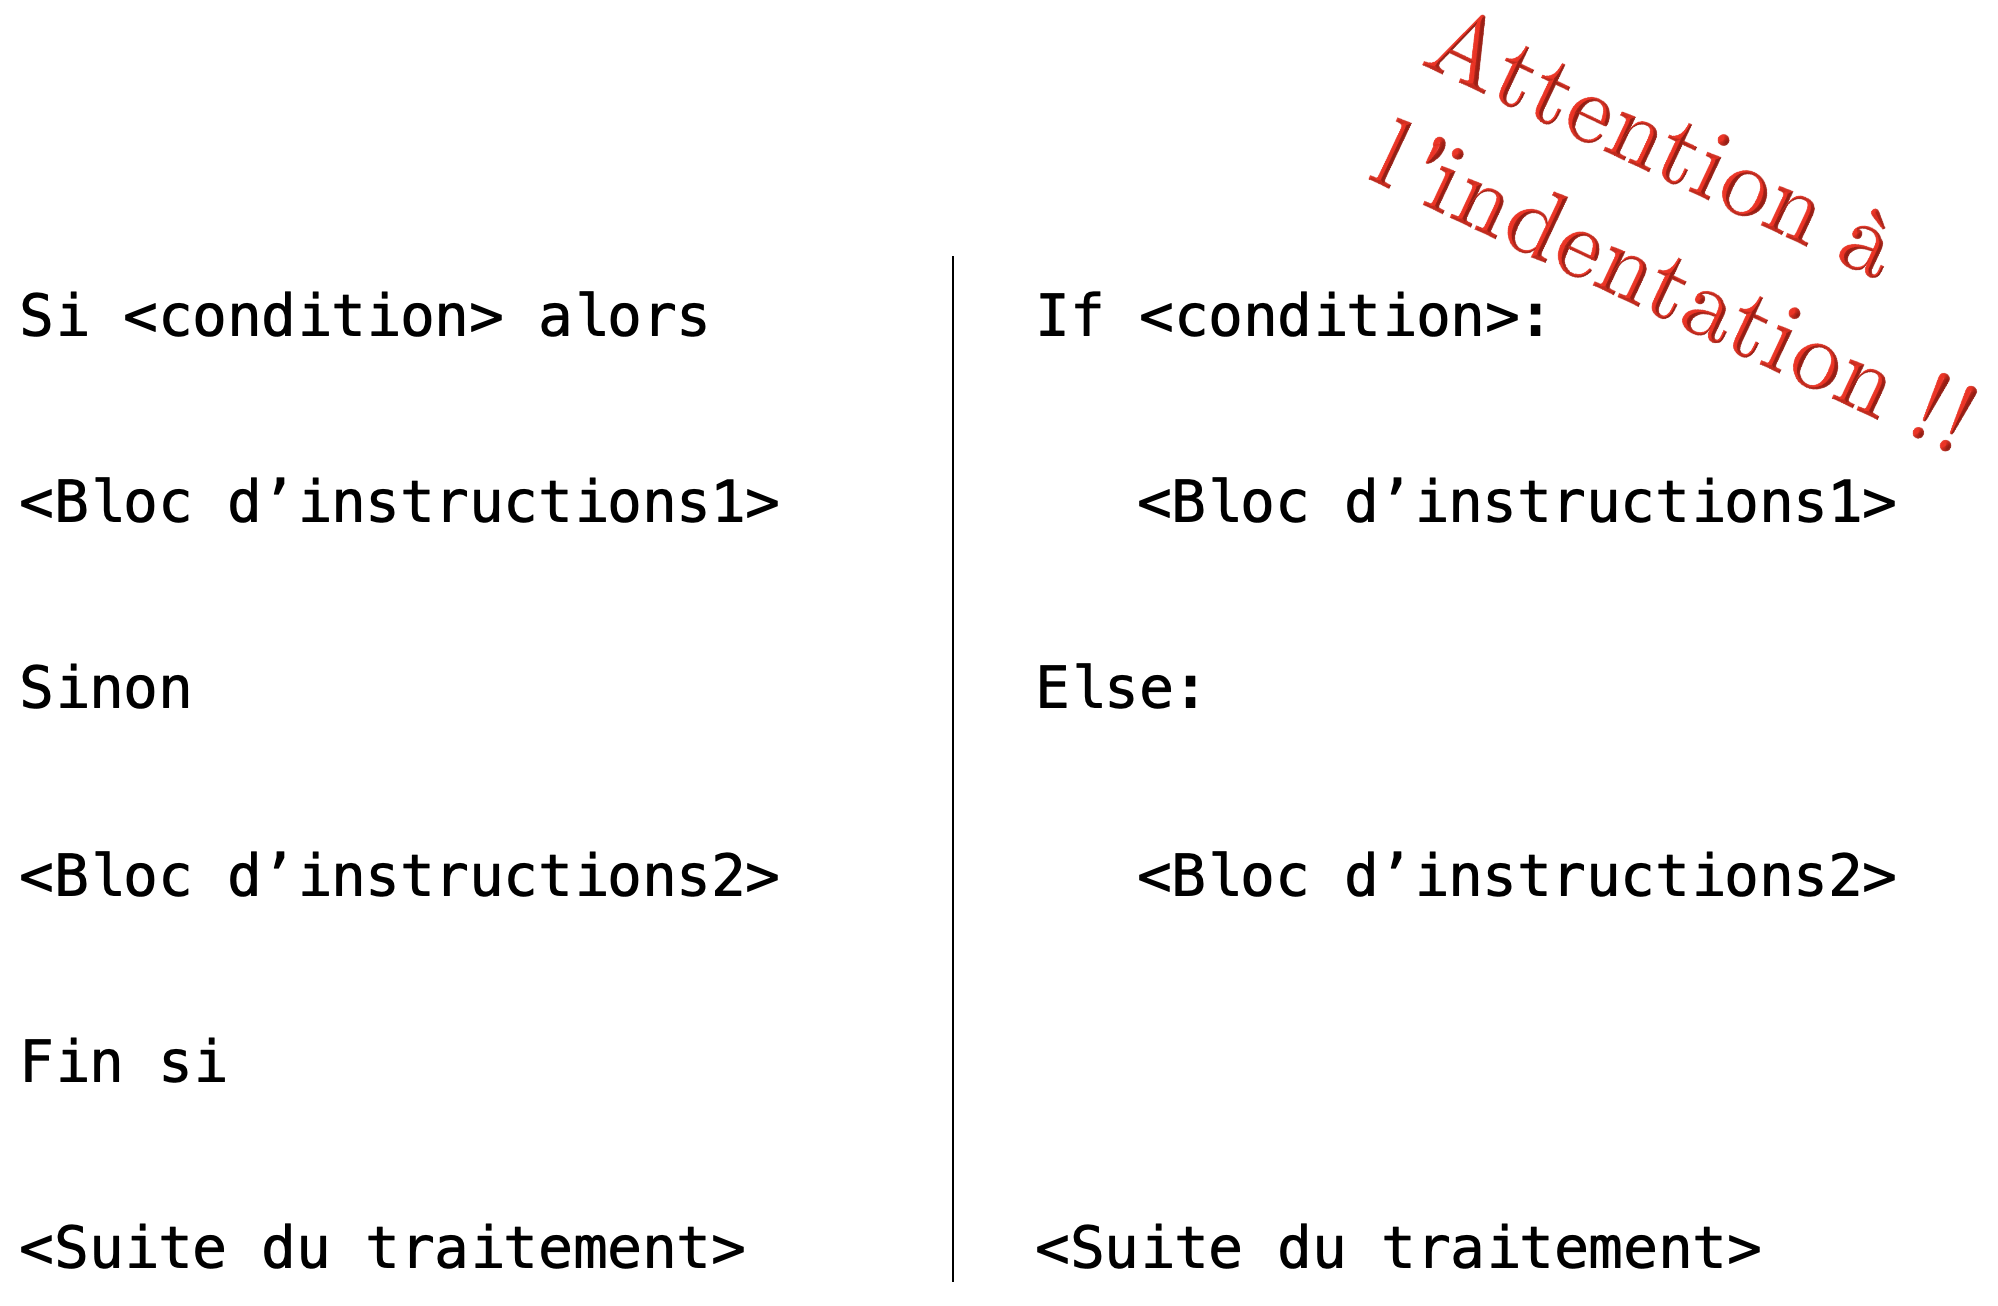
\includegraphics[width=0.8\textwidth]{014_IfThenElse.png}
	\end{figure}
	
	\begin{listing}[H]
		\inputminted
		[
		bgcolor = gray!15, % pas essentiel
		fontsize = \footnotesize,
		linenos = true % numéros de ligne
		]
		{python}
		{_code/004_IfThenElse.py}
	\end{listing}
	Ce qui donne:
	\begin{verbatim}
		a negatif
		Fin du test
	\end{verbatim}
	
	Et Python permet enfin d'envisager de multiples alternatives en utilisant la structure dite "sinon si":

	\begin{figure}[H]
		\centering
		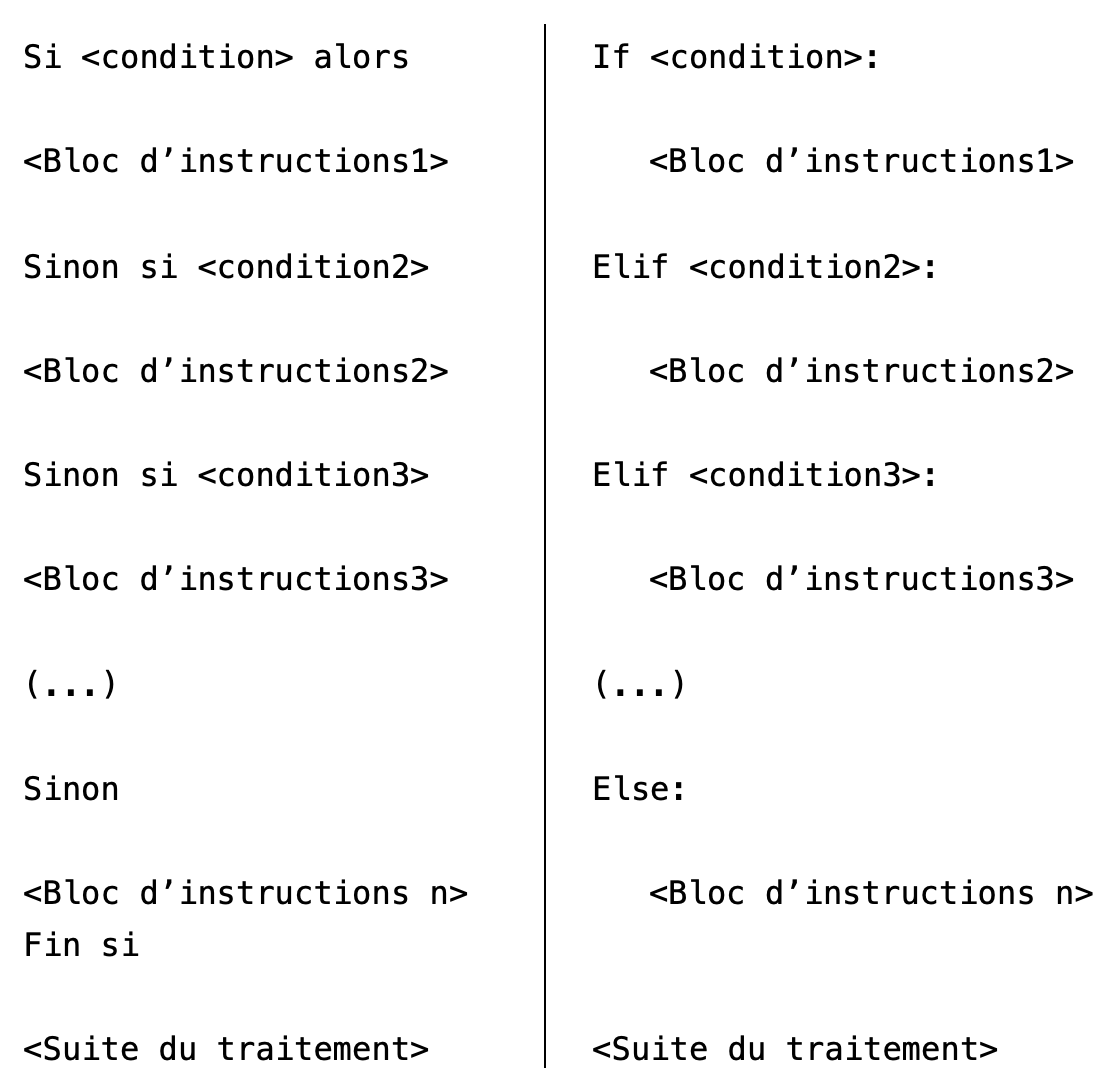
\includegraphics[width=0.8\textwidth]{015_Elif.png}
	\end{figure}
	
	\begin{tcolorbox}[colframe=red!75!black, boxrule=2pt]
		\begin{minipage}{1\textwidth}
			\begin{itemize}				
				\item Depuis votre ENT, lancez l'application "Capytale".
				\item Rejoignez l'activité que j'ai préparée pour la séance avec le code:
			\end{itemize}
			\centering
			\textbf{\texttt{5dc2-1885289}}
			\begin{itemize}				
				\item Une fois que vous avez fini cette activité je vous propose deux exercices supplémentaires facultatifs:
			\end{itemize}
			\centering
			\textbf{\texttt{d80d-1885381}}
		\end{minipage}
	\end{tcolorbox}
	
	\noindent
	\framebox{\parbox{\dimexpr\linewidth-2\fboxsep-2\fboxrule}{\centering \textbf{ATTENTION:} Comme on l'a vu dans l'activité, les calculs algébriques et les tests avec les nombres entiers (type int) sont tous exacts. En revanche, \textbf{il n'en est pas de même avec les nombres flottants} (type float): certains calculs sont exacts et d'autres non, de même pour les tests. Nous verrons plus loin dans le programme pourquoi il en est ainsi (c'est dû à la façon dont les nombres flottants sont représentés en binaire dans l'ordinateur). Ce qu'il faut retenir ici, c'est qu'il ne faut pas faire des tests d'égalité brutaux entre deux nombres flottants.}}
	
	\subsection{Boucles}
	\subsubsection*{Boucles itératives}
	Il nous arrive souvent de devoir répéter plusieurs fois la même opération --- dans la vie courante on peut penser à des exercices physiques (des pompes par exemple) ou des actes élémentaires comme mettre un article dans un caddie au supermarché ou encore arroser toutes les plantes d'un jardin. Dans tous ces cas on a une action de base identique qu'on va répéter --- soit dans exactement le même contexte (les pompes) soit en le faisant varier légèrement (le supermarché où on ne prend a priori pas n fois le même article).
	
	La même chose se produit en calculs et donc en programmation --- par exemple: on place une somme de 1000 euros sur un compte rémunéré à 2\% (on multiplie donc chaque année la somme disponible sur le compte par 1,02) et on aimerait savoir la somme dont on disposerait dans 10 ans.
	
	L'approche "brutale" consisterait à procéder ainsi:
	\begin{verbatim}
		somme0 = 1000
		somme1 = somme0 * 1.02
		somme2 = somme1 * 1.02
		somme3 = somme2 * 1.02
		...
	\end{verbatim}
	On pourrait l'améliorer légèrement en limitant le nombre de variables utilisées:
	\begin{verbatim}
		somme = 1000
		somme = somme * 1.02
		somme = somme * 1.02
		somme = somme * 1.02
		...
	\end{verbatim}
	Mais dans les deux cas on ferait 11 fois rigoureusement le même calcul --- et si soudain on nous demandait combien ça ferait au bout de 100 ans, on devrait le faire 101 fois!
	
	Solution pour éviter cet écueil: les \textbf{boucles itératives} ou \textbf{boucle pour} qui permet de répéter une séquence d'instructions un nombre fixé de fois:
	\begin{verbatim}
		Pour compteur allant de valeur_init à valeur_finale
		
		<Bloc d’instructions>
		
		Fin pour		
		
		<Suite du traitement>
	\end{verbatim}
	
	\leavevmode
	\\
	Ce qui, en syntaxe Python, s'écrit:
	
	\begin{verbatim}
		For compteur in range(valeur_init, valeur finale + 1):
		
		    <Bloc d’instructions>
		
		<Suite du traitement>
	\end{verbatim}
	
	\textit{(Et, évidemment, \textcolor{red}{\textbf{ATTENTION A L'INDENTATION!!}})}
	
	Quelques remarques au sujet de cette syntaxe:
	\begin{itemize}
		\item Si \texttt{
				valeur\_finale < valeur\_init}
			, il n’y a pas d'erreur: la boucle ne s’exécute simplement pas et on passe directement à la suite du traitement.
		\item En Python, l’instruction \texttt{
				range(valeur\_init, valeur\_finale + 1)} 
			définit une plage de \textbf{
				valeurs entières consécutives} 
			commençant à valeur\_init et se terminant à valeur\_finale (cette plage contient donc \texttt{
				(valeur\_finale – valeur\_init + 1}
			) valeurs – ce qui explique le "\texttt{+1}" dans la syntaxe. Ainsi:
		\begin{itemize}
			\item L'instruction \texttt{range(1,6)} correspond à la plage de valeurs \texttt{\{1, 2, 3, 4, 5\}}.
			\item L’instruction \texttt{range(0,3)} correspond à la plage de valeurs \texttt{\{0, 1, 2\}}.
			\item Dans le cas précédent où la valeur initiale est égale à 0, on peut l’omettre en n’écrivant que \texttt{range(valeur\_finale + 1)} soit, dans ce cas : \texttt{range(3)}.
		\end{itemize}
	\end{itemize}
	\leavevmode
	\\
	Pour revenir à notre problème des 1000 euros placés sur un compte rémunéré, la fonction suivante va renvoyer la somme demandée:
	
	\begin{figure}[H]
		\centering
		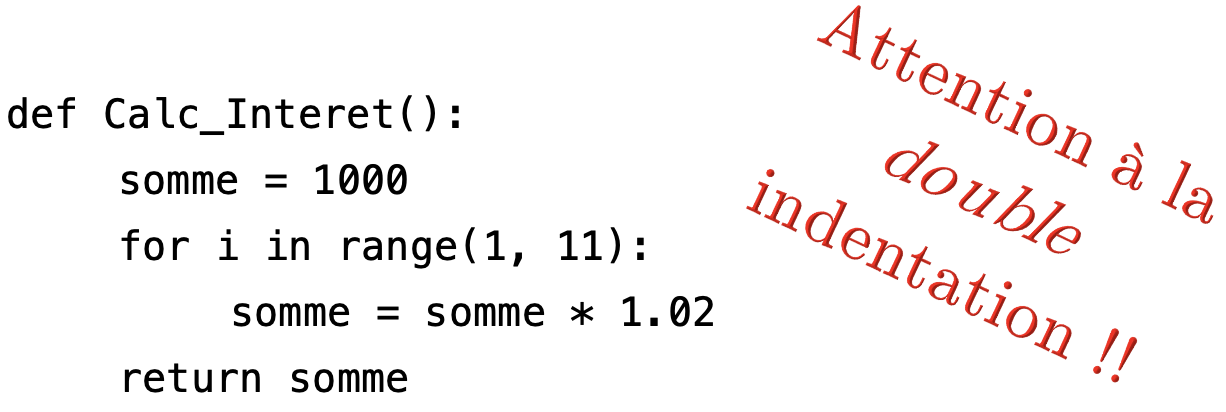
\includegraphics[width=0.6\textwidth]{016_CalcInteret.png}
	\end{figure}
	
	\begin{tcolorbox}[colframe=red!75!black, boxrule=2pt]
		\begin{minipage}{1\textwidth}
			\begin{itemize}				
				\item Depuis votre ENT, lancez l'application "Capytale".
				\item Rejoignez l'activité que j'ai préparée pour la séance avec le code:
			\end{itemize}
			\begin{center}
				\textbf{\texttt{1a11-1938165}}
			\end{center}
			\leavevmode
			\\
			\textbf{ATTENTION}: à partir de maintenant les exercices vont relever de la réelle programmation --- au sens "résolution d’un problème au moyen d’un programme" ce que vous allez trouver significativement plus difficile que ce que l’on a fait jusqu’à présent. Conseils, si vous avez du mal :
			\begin{itemize}				
				\item Prenez le temps de réfléchir mais ne restez pas bloqué\textperiodcentered e --- n’hésitez pas à demander de l’aide (à moi, à vos camarades...).
				\item Il n’y a aucun secret: "plus on code, meilleur on sera". Entrainez-vous le plus possible en utilisant les notebooks fournis en séance, mais aussi France IOI (que je regarderai de temps en temps).
			\end{itemize}
		\end{minipage}
	\end{tcolorbox}

	\subsubsection*{Boucles conditionnelles}
	Reprenons l’exemple de la section précédente du placement de 1000 euros sur un compte rémunéré à 2\% (on multiplie donc chaque année la somme disponible sur le compte par 1,02). Cette fois, au lieu de déterminer la somme disponible après un certain nombre d'années, on cherche à calculer le nombre d'années qu'il faudrait attendre avant de disposer d'au moins 2000 euros.
	
	On va donc de nouveau effectuer une boucle sur le calcul "\texttt{somme = somme * 1.02}" sauf que cette fois on ne sait pas à l’avance combien de fois on va faire le calcul --- ce nombre de fois est même précisément ce que l'on cherche à calculer. Nous allons donc répéter l'opération jusqu’à ce qu'une condition ("\texttt{somme >= 2000}") soit remplie. En algorithmique, cette démarche s’appelle \textbf{boucle conditionnelle} ou encore \textbf{boucle tant que}:
	
		\begin{verbatim}
		Tant que <condition vraie>
		
		<Bloc d’instructions>
		
		Fin tant que
		
		<Suite du traitement>
	\end{verbatim}
	
	\leavevmode
	\\
	Ce qui, en syntaxe Python, s'écrit:
	
	\begin{verbatim}
		While <condition vraie>:
		
		    <Bloc d’instructions>
		
		<Suite du traitement>
	\end{verbatim}
	
	\textit{(Et, encore et toujours, \textcolor{red}{\textbf{ATTENTION A L'INDENTATION!!}})}
	
	Pour revenir à notre problème des 1000 euros placés sur un compte rémunéré, la fonction suivante va renvoyer le nombre d’années:
	
	\begin{figure}[H]
		\centering
		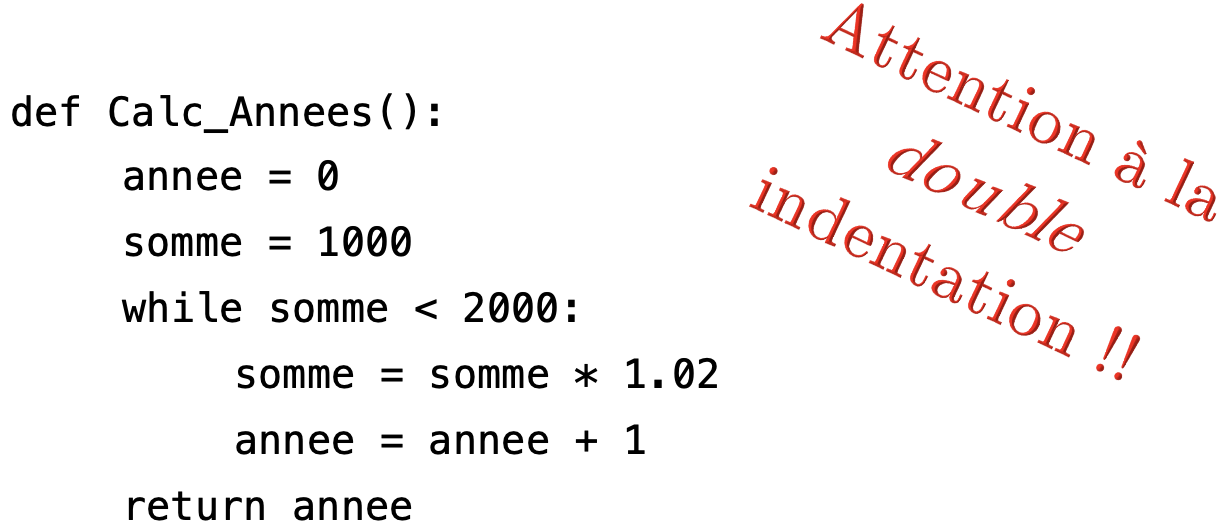
\includegraphics[width=0.6\textwidth]{017_CalcAnnees.png}
	\end{figure}
	
	\textbf{ATTENTION} à la définition des boucles tant que --- considérez la fonction ci-dessous:
	\begin{listing}[H]
		\inputminted
		[
		bgcolor = gray!15, % pas essentiel
		fontsize = \footnotesize,
		linenos = true % numéros de ligne
		]
		{python}
		{_code/005_BoucleInfinie.py}
	\end{listing}
	Que va-t-il se passer si je fais un appel à cette fonction essai\_boucle?
	
	La condition \texttt{i = 100} ne sera \textbf{\textit{jamais}} remplie puisque i est initié (ligne 2) à 1 puis est incrémenté dans la boucle (ligne 4) de 2 en 2 --- et ne prendra donc jamais que des valeurs impaires. Donc la condition "\texttt{i != 100}" sera \textit{toujours} vraie, et on a donc défini \textbf{une boucle infinie} --- qui soit ne terminera jamais (ce sera le cas dans le cas d'un traitement simple comme celui-ci) et nécessitera une intervention manuelle de l'utilisateur pour être arrêtée, soit va à terme (dans des cas plus complexes) engendrer un dépassement de capacité et donc faire planter le programme. Il faut donc toujours bien vérifier que la condition du "tant que" va, à un moment donné, devenir fausse.
	
	\begin{tcolorbox}[colframe=red!75!black, boxrule=2pt]
		\begin{minipage}{1\textwidth}
			\begin{itemize}				
				\item Depuis votre ENT, lancez l'application "Capytale".
				\item Rejoignez l'activité que j'ai préparée pour la séance avec le code:
			\end{itemize}
			\centering
			\textbf{\texttt{88a7-1939474}}
		\end{minipage}
	\end{tcolorbox}
	
	\pagebreak
	
	\section{Types de données construits}
	Jusqu'à présent nous n'avons manipulé que des types de données simples: des entiers, des flottants, des chaines de caractères, des booléens.
	
	En informatique, comme dans la vie courante, ces types de données sont rarement suffisants --- il nous est nécessaire de considérer des ensembles de données unis entre eux: c'est ce qu'on appelle des types de données construits (par opposition aux types de données simples, donc) --- et c'est ce que nous allons étudier à présent.
	\subsection{Listes}
	\subsubsection*{Introduction}
	Si on désire étudier l'évolution d’un prix sur plusieurs années, on ne va pas regarder uniquement un prix en particulier, mais l'ensemble des prix sur la période. Il faut donc être capable de stocker toutes ces valeurs dans une même structure afin de pouvoir y accéder sans difficulté.
	
	La structure la plus simple que l'on puisse utiliser est un tableau (en général unidimensionnel, c’est-à-dire avec une seule ligne):
	
	\begin{figure}[H]
		\centering
		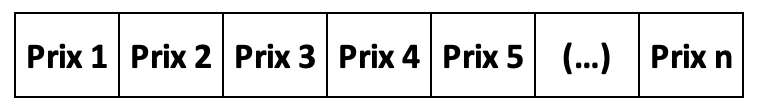
\includegraphics[scale=0.5]{018_TabUniDim.png}
	\end{figure}	

	En Python, un tableau est assimilé à une structure spécifique appelée liste (de type \texttt{list}).
	
	\noindent
	\framebox{\parbox{\dimexpr\linewidth-2\fboxsep-2\fboxrule}{Une \textbf{liste} est une \textbf{collection ordonnée} (ou séquence) d’éléments encadrée par des \textbf{crochets}, les éléments étant séparés par des \textbf{virgules}.}}
	
	\texttt{[1, 2, -5, 10]} est une liste de quatre éléments; \texttt{["M", "a", "r", "c"]} en est une également; tout comme \texttt{[99, "bonjour", -3, "\$"]}.  
	\\
	\\
	\\
	\noindent
	\framebox{\parbox{\dimexpr\linewidth-2\fboxsep-2\fboxrule}{La \textbf{longueur d’une liste}, qu’on peut obtenir avec la fonction \textbf{\texttt{len}}, est le nombre d’éléments qui la composent.}}
	
	\texttt{\textbf{len([1, 2, -5, 10])}} renverra la valeur 4.
	\\
	
	On peut initier / définir des listes de plusieurs manières :
	\begin{itemize}
		\item \textbf{Créer une liste vide:}
		\texttt{Lst1  =[]}
		\item \textbf{Créer une liste "par extension"}:
		\begin{itemize}
			\item Soit on la définit directement avec les éléments qui la composent:
				\begin{verbatim}
					Lst2 =[1, 3, -2, 10]
				\end{verbatim}
			\item Soit on y ajoute des éléments au fur et à mesure au moyen de la méthode (ou fonction) \texttt{append} qui prend en argument une variable et l'ajoute "au bout" d'une liste:
			\begin{verbatim}
				L = [1, 5, 8]
				L.append(150)
				L == [1, 5, 8, 150]
			\end{verbatim}
			renverra \texttt{True} parce que le \texttt{append} aura ajouté la valeur 150 après le dernier élément de la liste.
		\end{itemize}
		\item Deux autres approches --- \textbf{"par transtypage"} et \textbf{"par compréhension"} seront couvertes plus loin dans ce cours.		
	\end{itemize}
	\leavevmode
	\\
	
	Considérons quelques caractéristiques de ces listes:
	\begin{itemize}
		\item On peut effectuer divers \textbf{tests sur des listes}:
		\begin{itemize}
			\item Test d'\textbf{égalité}: \texttt{[1, 2, 3] == [1, 2, 3]} renverra \texttt{True} puisque les deux listes sont égales.
			\item Test d'\textbf{inégalité}: \texttt{[1, 2, 3] != [1, 3, 2]} et \texttt{[1, 2, 3] != [1, 2, 3, 4]} renverront tous les deux \texttt{True} puisque les listes ne sont pas strictement égales entre elles.
			\item Test d'\textbf{appartenance} au moyen du mot clé "\texttt{in}": \texttt{2 in [1, 2, 3]} renverra donc \texttt{True}.
			\item Et à l'inverse, test de "\textbf{non appartenance}" en utilisant l'opérateur logique \texttt{not} que l'on a déjà vu: \texttt{5 not in [1, 2, 3]} renverra \texttt{True}.
		\end{itemize}
		\item Les éléments d'une liste sont des \textbf{variables} - on peut donc les manipuler de la même manière que des variables, et notamment les \textbf{(ré) affecter}. Par exemple:
		\begin{verbatim}
			L = [1, 2, -5, 10]
			L[2] = 0
			L == [1, 2, 0, 10]
		\end{verbatim}
		renverra \texttt{True} puisqu'on aura "remplacé" la valeur -5 par la valeur 0 dans L[2].
		\item \textbf{Indexation}:
		\begin{itemize}
				\begin{figure}[H]
					\centering
					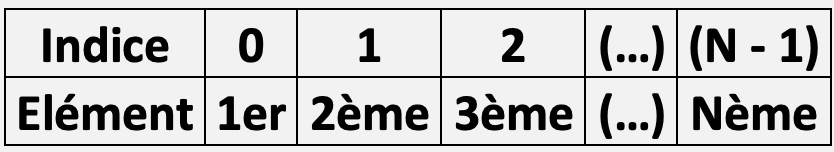
\includegraphics[scale=0.2]{019_LstIndex.jpg}
				\end{figure}	
			\item Le premier élément a pour indice 0;
			\item Le second a pour indice 1;
			\item (...)
			\item Le n\textsuperscript{ème} a pour indice (n-1).
		\end{itemize}
		\item A l'inverse, pour \textbf{trouver un élément} dans la liste:
			\begin{itemize}
				\item  L’élément d'indice j d'une liste L est défini par l'instruction \texttt{L[j]}. 
				\leavevmode
				\\Exemple: on considère la liste \texttt{L = [1, 2, -5, 10]}. Alors:
				\begin{itemize}
					\item \texttt{L[0]} correspond à "1";
					\item \texttt{L[2]} correspond à "-5";
					\item etc...
					
				\end{itemize}
			\end{itemize}
			Remarque: si on veut accéder à un indice qui n'existe pas, on déclenche une erreur de type
			\begin{center}
				\texttt{IndexError: list index out of range}
			\end{center}
			c'est-à-dire que l'on a voulu utiliser un indice en dehors de la plage autorisée (de 0 jusqu'à \texttt{len} - 1).			
			\begin{itemize}
				\item On peut effectuer des \textbf{opérations} sur des listes au moyen d'opérateurs --- \textbf{\textit{qu'il ne faut pas confondre avec les opérateurs arithmétiques utilisant les mêmes symboles}}:
				\begin{itemize}
					\item L'opérateur "\texttt{+}" est un \textbf{opérateur de concaténation} --- il permet de rassembler deux listes: l'instruction \texttt{[1, 2] + [3]} renvoie la liste \texttt{[1, 2, 3]}.
					\item L'opérateur "\texttt{*}" est un \textbf{opérateur de duplication} --- il permet de dupliquer plusieurs fois une liste pour en créer une autre: l'instruction \texttt{[1] * 3} renvoie la liste \texttt{[1, 1, 1]}; l'instruction \texttt{[1, 2] * 2} renvoie la liste \texttt{[1, 2, 1, 2]}.
				\end{itemize}
			\end{itemize}
	\end{itemize}
	
		\begin{tcolorbox}[colframe=red!75!black, boxrule=2pt]
		\begin{minipage}{1\textwidth}
			\begin{itemize}				
				\item Depuis votre ENT, lancez l'application "Capytale".
				\item Rejoignez l'activité que j'ai préparée pour la séance avec le code:
			\end{itemize}
			\begin{center}
				\textbf{\texttt{7b7d-2075987}}
			\end{center}
			\begin{itemize}
				\item \textit{Si vous avez terminé l'activité ci-dessus, penchez-vous sur une série d'exercices supplémentaires plus sophistiqués en utilisant le code:}
			\end{itemize}
			\begin{center}
				\textit{\textbf{\texttt{28b9-2076098}}}
			\end{center}
			
		\end{minipage}
	\end{tcolorbox}
	
	
%	On peut aussi créer une liste « par compréhension » – on la définit alors à partir d’une fonction qui va la constituer selon la syntaxe suivante :
%	[fonction(i) for i in range(valeur initiale, valeur finale + 1) if condition(i)]
%	Ainsi on peut envisager les deux exemples suivants :
%	•	[i for i in range(5)] correspond à la liste [0, 1, 2, 3, 4].
%	•	[i**2 for i in range(5) if i%2 == 1] correspond à la liste [1, 9].
%	
%	
\end{document}

%Eléments manquants:
%- Tests d'assertions
%- Listes par copmpréhension
%- Copies de listes (voir la fin de l'activité de Poulmaire NSI Première Partie 1 Chapitre 6 Listes définition et indexation)